\documentclass[a4paper,table,dvipsnames]{article}
\usepackage{lmodern}
\usepackage[utf8]{inputenc}
\usepackage[T1]{fontenc}
\usepackage[english]{babel}
\usepackage{latexsym}
\usepackage{amsmath,amsfonts,amssymb}
\usepackage{mathpartir}
\usepackage{amsthm}
\usepackage{tikz}
\usepackage{enumitem}
\usepackage[probability,adversary,sets,operators,primitives]{cryptocode}
\usepackage{fancyhdr}
\usepackage{hyperref}
\usepackage{wrapfig}
%\usepackage[table]{xcolor}
%\usepackage[margin=2.7in]{geometry}

\pagestyle{fancy}
\usetikzlibrary{shapes,arrows,positioning}
\tikzstyle{vertex} = [draw, circle]

\theoremstyle{definition}
\newtheorem{definition}{Definition}[section]
\newtheorem{remark}{Remark}
\newtheorem{lemma}{Lemma}
\newtheorem{claim}{Claim}
\newtheorem{conjecture}{Conjecture}
\newtheorem{construction}{Construction}
\newtheorem{theorem}{Theorem}
%\newtheorem*{theorem}{Theorem}
\newtheorem{example}{Example}
\newtheorem{hint}{Hint}
\setlength{\parindent}{0ex}

\rhead[Lecture Notes 4]{Lecture Notes 4}
\lhead[CS-E4340 Cryptography, Chris Brzuska]{CS-E4340 Cryptography, Chris Brzuska}

\newcommand{\M}[1]{\ensuremath{\text{\texttt{#1}}}}
\renewcommand{\O}[1]{\ensuremath{\mathsf{#1}}}
\newcommand{\pcvar}[1]{\ensuremath{\mathit{#1}}}
%\newcommand{\pcassert}{\ensuremath{\mathbf{assert}\;}}
\newcommand{\pckw}[1]{\highlightkeyword{#1}}
\newcommand{\pctype}[1]{\mathsf{#1}}
\newcommand{\ininterface}[1]{[#1\rightarrow]} %{I^{in}_{#1}}
\newcommand{\outinterface}[1]{[\rightarrow#1]} %{I^{out}_{#1}}
\newcommand{\m}{\pcvar{m}} %{I^{out}_{#1}}
\renewcommand{\verify}{\ver}
\newcommand{\ver}{\O{ver}} %{I^{out}_{#1}}
\renewcommand{\mac}{\O{mac}}
\renewcommand{\circ}{\rightarrow}

\newcommand\defeq{\mathrel{\overset{\makebox[0pt]{\mbox{\normalfont\tiny\sffamily
def}}}{=}}}
\def\checkmark{\tikz\fill[scale=0.4](0,.35) -- (.25,0) -- (1,.7) --
(.25,.15) -- cycle;}

\title{Lecture 4}
\author{Chris Brzuska}
\date{\today}

\begin{document}





This lecture covers \emph{message-authentication codes} and their security.

\section{Games, packages and reductions}
Recall that last week, we defined pseudorandom functions. Let us recall their definition.
\begin{definition}[Security of PRFs]\label{def:mono}
A $(\lambda,\lambda)$-PRF $f$ is \emph{secure} if for all probabilistic poly-time (PPT) adversaries $\adv$, the advantage
\[\mathsf{Adv}^{\M{Gprf}_f^0,\M{Gprf}^1}_{f,\adv}:=\abs{\prob{1=\adv\stackrel{\O{EVAL}}{\rightarrow}\M{Gprf}^0_f}-
\prob{1=\adv\stackrel{\O{EVAL}}{\rightarrow}\M{Gprf}^1_f}}\]
is negligible in $\lambda$, where $\M{Gprf}_f^0$ and $\M{Gprf}^1$ are defined in Figure~\ref{fig:PRGCODE}.
\end{definition}
In last week's lecture notes, we already discussed that we can consider \emph{games} as formal objects with
a \emph{parameters}, \emph{state} and \emph{oracles} which they provide. We write $[\rightarrow \M{G}]$ for the
oracles which a game $\M{G}$ provides, or, more precisely, the \emph{names} of the oracles which a game provides
 to the adversary, e.g.,
\[[\rightarrow\M{Gprf}_f^0]=\{\O{EVAL}\}=[\rightarrow\M{Gprf}^1].\]
Why are packages useful? Well, in this lecture, we will introduce the notion of a \emph{reduction} formally,
and a reduction is, perhaps surprisingly, a \emph{package}. Why is a reduction a package? Well, a reduction is
something that turns an adversary against one \emph{problem} into an adversary against another \emph{problem}.

\begin{wrapfigure}{R}{0.6\textwidth}
\vspace{-0.5cm}
\begin{center}
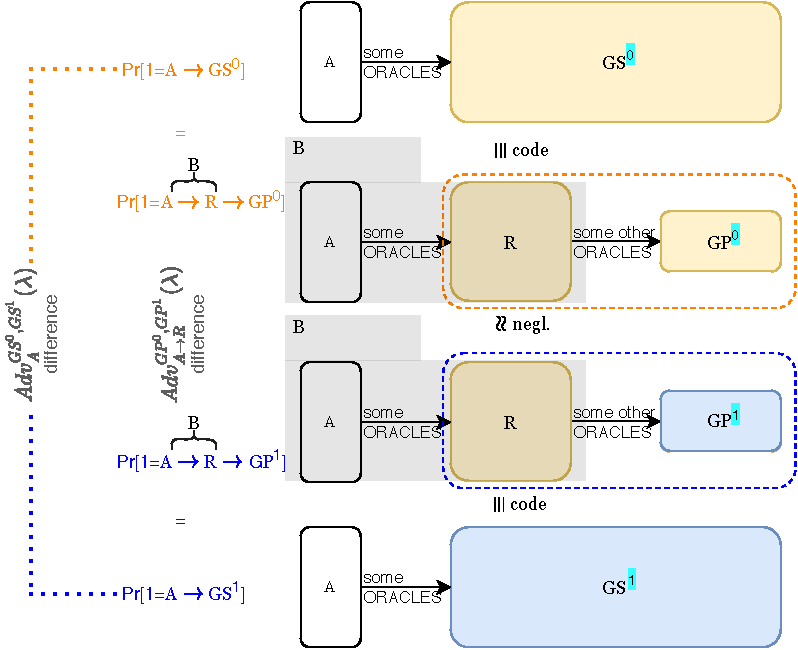
\includegraphics[width=0.6\textwidth]{reduction}
\caption{\label{fig:reduction-example}New adversary $\M{B}=\adv\circ\M{R}$}
\end{center}
\vspace{-0.5cm}
\end{wrapfigure}

\paragraph{Reductions}
Let's say that we want to prove the security of some system $S$, under the assumption that primitive $P$ is secure. In a reduction proof, we do this via a \emph{proof by contradiction} (which can take some time to get used to): we assume that $S$ is \emph{insecure} and prove that $P$ is then also insecure. If we can carry out such a proof, we can then argue that $S$ is secure. After all, if $S$ were insecure, then our proof would say that $P$ is also insecure, but this in contradiction to our assumption that $P$ is \emph{secure}.

So, how do we prove that $S$ being insecure implies $P$ being insecure? Here it is important to realize what it means for $S$ to be insecure. It means that there is some (efficient) adversary $\adv$ that can break the security of $S$. Similarly, to prove that $P$ is insecure, we have to provide a new efficient adversary $\M{B}$ that can break it. However, due to our assumption, we are allowed to use $\adv$ in the code of $\M{B}$. Note that we don't know the \emph{code} of $\adv$, so $\M{B}$ can only use $\adv$ in a black-box way, and we can't make any assumptions about the precise functioning of $\adv$.

Thus, we construct adversary $\M{B}$ as a \emph{composition} of $\adv$ and a package $\M{R}$, the latter of which we call reduction. To practice our notation, we will have that $\M{B}$ is code-equivalent to the composition $\adv\rightarrow\M{R}$, written $\M{B}\stackrel{\text{code}}{\equiv}\adv\rightarrow\M{R}$, and we'll have matching \emph{oracles} and \emph{dependencies}, which we write as $[\adv\rightarrow]=[\rightarrow\M{R}]$.

Reductions can be described explicitly, by defining reduction $\M{R}$ in pseudocode. Let us make this more explicit.
For simplicity, let us consider that the security of $P$ is defined as the indistinguishability between a real game $\M{GP}^0$
and an ideal game $\M{GP}^1$. Let us further consider that the security of $S$ is defined as the indistinguishability between
a real game $\M{GS}^0$ and an ideal game $\M{GS}^1$. Then a reduction $\M{R}$ from the security of $S$ to the security of $P$
is an (efficient!) package $\M{R}$ such that
\begin{align}
\notag          &\M{GS}^0\stackrel{\text{code}}{\equiv}\M{R}\rightarrow\M{GP}^0\text{ and }\\
\label{lalaland}&\M{GS}^1\stackrel{\text{code}}{\equiv}\M{R}\rightarrow\M{GP}^1.
\end{align}
With Equation~\ref{lalaland} at hand, we can prove\footnote{See Lecture Notes 3 and Lecture Video 4, minutes 16:30 and 27:56, for a concrete such argument: The main reason that code equivalence implies that two games behave exactly the same and thus, and adversary has exactly the same probability against the two games. We use this argument a lot in this course.}  that for all adversaries $\adv$, it holds that 
\begin{equation}\label{lalaland1}
\mathsf{Adv}^{\M{GS}^0,\M{GS}^1}_\adv(\lambda)=\mathsf{Adv}^{\M{GP}^0,\M{GP}^1}_{\adv\rightarrow\M{R}}(\lambda),
\end{equation}
and thus, if there is an efficient adversary $\adv$ which has non-negligible advantage against the pair $(\M{GS}^0,\M{GS}^1)$,
then there is also an efficient adversary $\adv\rightarrow\M{R}$ against the pair $(\M{GP}^0,\M{GP}^1)$ which has the same
advantage. However, we assume that there is no efficient $\bdv$ with non-negligible advantage $\mathsf{Adv}^{\M{GP}^0,\M{GP}^1}_{\bdv}$, thus taking $\bdv=\adv\rightarrow\M{R}$ leads to a contradiction. In conclusion, there cannot be an efficient $\adv$ such that $\mathsf{Adv}^{\M{GS}^0,\M{GS}^1}_\adv$ is non-negligible.

The \emph{core argument}, here, is that (1) $\adv\rightarrow\M{R}$ is efficient (i.e., PPT) whenever $\adv$ is efficient, and (2) Equation~\ref{lalaland1}. Before we can state the notion of a reduction formally, let us actually reflect on whether we needed Equation~\ref{lalaland1}, as an equality between advantage statements. Actually, we only need an argument which justifies that if $\mathsf{Adv}^{\M{GS}^0,\M{GS}^1}_\adv$ is non-negligible, then $\mathsf{Adv}^{\M{GP}^0,\M{GP}^1}_{\adv\rightarrow\M{R}}$ is non-negligible. Any of the following inequalities would establish the desired result:
\begin{align*}
\mathsf{Adv}^{\M{GS}^0,\M{GS}^1}_\adv(\lambda)&\leq\mathsf{Adv}^{\M{GP}^0,\M{GP}^1}_{\adv\rightarrow\M{R}}(\lambda)\\
\mathsf{Adv}^{\M{GS}^0,\M{GS}^1}_\adv(\lambda)&\leq 2\cdot\mathsf{Adv}^{\M{GP}^0,\M{GP}^1}_{\adv\rightarrow\M{R}}(\lambda)\\
\mathsf{Adv}^{\M{GS}^0,\M{GS}^1}_\adv(\lambda)&\leq \O{poly}(\lambda)\cdot\mathsf{Adv}^{\M{GP}^0,\M{GP}^1}_{\adv\rightarrow\M{R}}(\lambda)\\
\mathsf{Adv}^{\M{GS}^0,\M{GS}^1}_\adv(\lambda)&\leq \O{poly}(\lambda)\cdot\sqrt{\mathsf{Adv}^{\M{GP}^0,\M{GP}^1}_{\adv\rightarrow\M{R}}(\lambda)}\\
\mathsf{Adv}^{\M{GS}^0,\M{GS}^1}_\adv(\lambda)&\leq \O{poly}(\lambda)\cdot\sqrt[5]{\mathsf{Adv}^{\M{GP}^0,\M{GP}^1}_{\adv\rightarrow\M{R}}(\lambda)}
\end{align*}
The reason that all of these inequalities work is that multiplying (or dividing) by constants, polynomials and squaring (or taking square roots), a negligible function cannot become non-negligible (or vice versa). We are almost ready to state the notion of a reduction, but actually, we still need to make this statement a bit more general. The reason is that often, we have more than one algorithm $\M{R}$, and, e.g., might have inequalities such as 
\begin{equation}\label{lalaland12}
\mathsf{Adv}^{\M{GS}^0,\M{GS}^1}_\adv(\lambda)=\mathsf{Adv}^{\M{GP}^0,\M{GP}^1}_{\adv\rightarrow\M{R}_1}(\lambda)+\mathsf{Adv}^{\M{GP}^0,\M{GP}^1}_{\adv\rightarrow\M{R}_2}(\lambda),
\end{equation}
for two different, efficient $\M{R}_1$ to $\M{R}_1$. This equation still suffices, since the sum of two negligible functions is negligible again, and if $\mathsf{Adv}^{\M{GS}^0,\M{GS}^1}_\adv$ was non-negligible, then $\mathsf{Adv}^{\M{GP}^0,\M{GP}^1}_{\adv\rightarrow\M{R}_1}$ or 
$\mathsf{Adv}^{\M{GP}^0,\M{GP}^1}_{\adv\rightarrow\M{R}_2}$ would need to be non-negligible. As you can imagine, we can also combine this flexibility: Have \emph{several} efficient $\M{R}_i$ and some complex equation. To jump ahead, let me already mention the equation which we will see shortly:
\begin{align}
   \notag&\mathsf{Adv}^{\M{Gunf\text{-}cma}_{\m_f}^0,\M{Gunf\text{-}cma}_{\m_f}^1}_{\m_f,\adv}(\lambda)\\
   \label{lalaland123}&\quad\leq\mathsf{Adv}^{\M{Gprf}^0,\M{Gprf}^1}_{f,\adv\rightarrow\M{R}_1}(\lambda)+\mathsf{Adv}^{\M{Gprf}^0,\M{Gprf}^1}_{f,\adv\rightarrow\M{R}_2}(\lambda)+\frac{\O{poly}_{\adv}(\lambda)}{2^\lambda}
\end{align}
Here, we add two advantages and some negligible term $\frac{\O{poly}_{\adv}(\lambda)}{2^\lambda}$, where $\O{poly}_{\adv}$ is
some polynomial which depends on the adversary (in this case an upper bound on the number of queries that $\adv$ makes).
Thus, also Inequality~\ref{lalaland123} suffices to establish that if there is no efficient adversary such that 
\[\mathsf{Adv}^{\M{Gprf}_f^0,\M{Gprf}_f^1}_{f,\bdv}\] is non-negligible, then there is also no efficient adversary such
that \[\mathsf{Adv}^{\M{Gunf\text{-}cma}_{\m_f}^0,\M{Gunf\text{-}cma}_{\m_f}^1}_{\m_f,\adv}\] is non-negligible.

\begin{quote}
How do we know which combination is the right one in which situation?
\end{quote}

We don't really know this. Moreover, there are
often more than one right way to do this. In essence, any approach that works is good, and we will see many such
examples of proofs in this course (and the advanced course) so we can build our \emph{cryptographer's toolkit}, i.e., 
a list of many examples for how to do proofs. We will not go in too many proof techniques in this course, since we
balance seeing proof techniques with seeing concepts, and we focus more on concepts than on proof techniques in this
course. Nevertheless, we'll see many examples of proofs so they will hopefully become familiar over time.

Let us now state the notion of a reduction:
\begin{definition}[Reduction]
We call a package $\M{R}$ a reduction from the indistinguishability of $\M{GS}^0$ and  $\M{GS}^1$ to the indistinguishability of 
$\M{GP}^0$ and  $\M{GP}^1$, if
\begin{itemize}
\item $\M{R}$ is efficient, i.e., probabilistic polynomial-time (PPT), and
\item for any efficient adversary $\adv$, it holds that if $\mathsf{Adv}^{\M{GS}^0,\M{GS}^1}_\adv$ is non-negligible, then
      $\mathsf{Adv}^{\M{GP}^0,\M{GP}^1}_{\adv\rightarrow\M{R}}$ is non-negligible.
\end{itemize}
Additionally, we call two packages $\M{R}_1$ and $\M{R}_2$ reductions from the indistinguishability of $\M{GS}^0$ and  $\M{GS}^1$ to the indistinguishability of 
$\M{GP}^0$ and  $\M{GP}^1$, if
\begin{itemize}
\item $\M{R}$ is efficient, i.e., probabilistic polynomial-time (PPT), and
\item for any efficient adversary $\adv$, it holds that if $\mathsf{Adv}^{\M{GS}^0,\M{GS}^1}_\adv$ is non-negligible, then
      $\mathsf{Adv}^{\M{GP}^0,\M{GP}^1}_{\adv\rightarrow\M{R}_1}$ or $\mathsf{Adv}^{\M{GP}^0,\M{GP}^1}_{\adv\rightarrow\M{R}_2}$ is non-negligible.
\end{itemize}
In this case, we refer to $\M{R}_1$ and $\M{R}_2$ as a reductions, even though one of them alone does not match the first
part of the definition.
\end{definition}

\begin{wrapfigure}{R}{0.28\textwidth}
\vspace{-0.3cm}
		\begin{pcvstack}
		\underline{\underline{$\M{Key}$}}\\
                                \\
		\procedure{$\O{GET}()$}{
			\pcif k=\bot:\\
			\pcind k\sample \bin^\lambda\\
			\pcreturn k}
			\pcvspace
              \procedure{Package Param.}{
				\lambda\text{:} \< \quad \text{security par.}
			              }
										\pcvspace
									\procedure{Package State}{
				k\text{:} \< \quad \text{key}
			              }
		\end{pcvstack}
\vspace{-0.5cm}
\end{wrapfigure}


\paragraph{Key Packages}
One useful package which we will use a lot is the $\M{Key}$ package. We will externalize the key of a package into
a package in order to make the main package(s) of a game stateless. Let us see this on the example of the games $\M{Gprf}_f^0$
and $\M{Gprf}_f^1$. We will split game $\M{Gprf}_f^0$ into two packages, $\M{Key}$ (given in the figure on the right
of this page) and $\M{Prf}^0$ (given in Figure~\ref{fig:PRGCODE}). When we \emph{inline} the code of $\M{Key}$ into
$\M{Prf}^0$, then we obtain $\M{Gprf}_f^0$ again. We call merging two packages in this way \emph{inlining} and we
call the converse process, i.e. splitting a package into two, \emph{outlining}, since it is the reverse of inlining.

One important observation of splitting a game into two is that the security definition is equivalent to the original one, i.e., both security definitions are satisfied by the same functions. Let us prove this on the example of the PRF security game.
Let us start by formulating a modular version of the definition, using the $\M{Key}$ package we just defined.

\begin{figure}
\begin{center}
  \begin{pcvstack}
    \begin{pchstack}
          \begin{pcvstack}
            \underline{\underline{$\M{Gprf}_f^0$}}\\
                \\
              \procedure{Package Parameters}{
				\lambda\text{:} \< \quad \text{security parameter}\\
				\pcvar{in}\text{:} \< \quad \text{input length}\;\lambda\\
			  f\text{:} \< \quad \text{function},\,(\pcvar{in},\lambda)\text{-PRF} 
			              }
										\pcvspace
										              \procedure{Package State}{
																	k\text{:} \< key
			              }
										\pcvspace
      \procedure{$\O{EVAL}(x)$}{
			 \pcassert x\in\bin^{\text{in}}\\
			 \pcif k=\bot:\\
			\pcind k\sample\bin^\lambda\\
        y\gets f(k,x)\\
        \pcreturn y}
    \end{pcvstack}
            \pchspace
    \begin{pcvstack}
            \underline{\underline{$\M{Gprf}^1$}}\\
                \\
              \procedure{Package Parameters}{
				\lambda\text{:} \< \quad \text{security parameter}\\
				\pcvar{in}\text{:} \< \quad \text{input length}\;\lambda\\
			              }
										\pcvspace
										              \procedure{Package State}{
				T\text{:} \< \quad \pckw{table}[\pctype{bitstring},\pctype{integer} \to \pctype{bitstring}] 
			              }
										\pcvspace
      \procedure{$\O{EVAL}(x)$}{
			 \pcassert x\in\bin^{\text{in}}\\
				\pcif T[x] = \bot\\
				\pcind T[x]\sample\bin^\lambda\\
				y\gets T[x]\\
        \pcreturn y}
		\end{pcvstack}
		\end{pchstack}
		\pcvspace
		\begin{pchstack}
		                   \begin{pcvstack}
            \underline{\underline{$\M{Prf}^0_f$}}\\
                \\
              \procedure{Package Parameters}{
				\lambda\text{:} \< \quad \text{security parameter}\\
				\pcvar{in}\text{:} \< \quad \text{input length}\;\lambda\\
				\pcvar{out}\text{:} \< \quad \text{output length}\;\lambda\\
			  f\text{:} \< \quad \text{function},\,(\pcvar{in},\pcvar{out})\text{-PRF} 
			              }
										\pcvspace
										              \procedure{Package State}{
																	\text{no state}
			              }
										\pcvspace
      \procedure{$\O{EVAL}(x)$}{
       \pcassert x\in\bin^{\text{in}}\\
	            k\gets\O{GET}\\
							\\
        y\gets f(k,x)\\
        \pcreturn y}
    \end{pcvstack}
            \pchspace
    \begin{pcvstack}
            \underline{\underline{$\M{Prf}^1$}}\\
                \\
              \procedure{Package Parameters}{
				\lambda\text{:} \< \quad \text{security parameter}\\
				\pcvar{in}\text{:} \< \quad \text{input length}\;\lambda\\
				\pcvar{out}\text{:} \< \quad \text{output length}\;\lambda\\
			              }
										\pcvspace
										              \procedure{Package State}{
				T\text{:} \< \quad \pckw{table}[\pctype{bitstring},\pctype{integer} \to \pctype{bitstring}] 
			              }
										\pcvspace
      \procedure{$\O{EVAL}(x)$}{
			 \pcassert x\in\bin^{\text{in}}\\
				\pcif T[x] = \bot\\
				\pcind T[x]\sample\bin^\lambda\\
				y\gets T[x]\\
        \pcreturn y}
		\end{pcvstack}		
	\end{pchstack}
		\end{pcvstack}		
	\end{center}
\caption{\label{fig:PRGCODE}The games $\M{Gprf}_f^0$ and $\M{Gprf}_f^1$ and the packages $\M{Prf}^0_f$ and $\M{Prf}^1$.}
\end{figure}

\begin{definition}[Modular Security of PRFs]\label{def:modular}
A $(\lambda,\lambda)$-PRF $f$ is \emph{secure according to the modular security definition for PRFs}
 if for all PPT  adversaries $\adv$, the advantage
\begin{align*}
  \mathsf{Adv}^{\M{Prf}_f^0\rightarrow\M{Key},\M{Gprf}^1}_{f,\adv}
:= \abs{\prob{1=\adv\stackrel{\O{EVAL}}{\rightarrow}\M{Prf}^0_f\stackrel{\O{GET}}{\rightarrow} \M{Key}}
  -\prob{1=\adv\stackrel{\O{EVAL}}{\rightarrow}\M{Gprf}^1}}
\end{align*}
is negligible in $\lambda$.
\end{definition}
With this definition at hand, we can now formulate the code equivalence between the composed game and the monolithic (i.e., single code-piece) game.
\begin{claim}[Code Equivalence]\label{claim:code-equiv}
\[\M{Prf}_f^0\stackrel{\O{GET}}{\rightarrow}\M{Key}\stackrel{\text{code}}{\equiv}\M{Gprf}_f^0\]
\end{claim}
From here, we obtain the equivalence of the two definitions, as formulated in the following statement.
\begin{claim}\label{claim:hopsdohops}
A $(\lambda,\lambda)$-PRF $f$ is \emph{secure} if and only if it is \emph{secure according to the modular security definition for PRFs}.
\end{claim}
Due to Claim~\ref{claim:hopsdohops}, for a PRF, from now on, we only use the term \emph{secure}, regardless of whether we aim to use Definition~\ref{def:mono} or Definition~\ref{def:modular} in a statement/proof.

Claim~\ref{claim:code-equiv} is shown by \emph{inlining} the Key package. In the following, we show how Claim~\ref{claim:hopsdohops} follows from Claim~\ref{claim:code-equiv}.

\begin{proof}
Let $\adv$ be an efficient adversary. Due to the code equivalence (Claim~\ref{claim:code-equiv}), we have that 
\begin{equation}\label{eq:previous}
\prob{1=\adv\stackrel{\O{EVAL}}{\rightarrow}\M{Gprf}^0_f}=\prob{1=\adv\stackrel{\O{EVAL}}{\rightarrow}\M{Prf}^0_f\stackrel{\O{GET}}{\rightarrow}\M{Key}}.
\end{equation}
Therefore,
\begin{align*}
\mathsf{Adv}^{\M{Gprf}_f^0,\M{Gprf}^1}_{f,\adv} &\stackrel{\text{def}}{=}\abs{\prob{1=\adv\stackrel{\O{EVAL}}{\rightarrow}\M{Gprf}^0_f}-\prob{1=\adv\stackrel{\O{EVAL}}{\rightarrow}\M{Gprf}^1}}\\
&\!\!\stackrel{\text{Eq.~\ref{eq:previous}}}{=}\abs{\prob{1=\adv\stackrel{\O{EVAL}}{\rightarrow}\M{Prf}^0_f\stackrel{\O{GET}}{\rightarrow}\M{Key}}-\prob{1=\adv\stackrel{\O{EVAL}}{\rightarrow}\M{Gprf}^1}}\\
&\stackrel{\text{def}}{=}\mathsf{Adv}^{\M{Prf}_f^0\rightarrow\M{Key},\M{Gprf}^1}_{f,\adv}
\end{align*}
Thus, $\mathsf{Adv}^{\M{Gprf}_f^0,\M{Gprf}^1}_{f,\adv}$ is negligible if and only if $\mathsf{Adv}^{\M{Prf}_f^0\rightarrow\M{Key},\M{Gprf}^1}_{f,\adv}$ is negligible.
\end{proof}


\section{PRFs imply PRGs}
We defined security of a PRG $g$ via an experiment where, if the secret bit $b=0$,
then the adversary receives $y:=g(x)$ for a uniformly random $x$, and if $b=1$, then
the adversary receives a uniformly random string $y$ of the same length as $g(x)$.
We can also security of PRGs via indistinguishability between two games, each of
which provide one oracle $\O{SAMPLE}$ which can only be queried once (this is ensured
via an $\pcassert$ in the beginning of the oracle---the oracle just checks whether it
has been called before.), and in
the real game ($b=0$), $\O{SAMPLE}$ samples a uniformly random $x$ and returns $y:=g(x)$,
whereas in the ideal game ($b=1$), $\O{SAMPLE}$ samples a uniformly random string $y$
of the same length as $g(x)$. We now define the games and PRG security formally.

\begin{definition}[PRG Security]
A PRG $g$ with stretch $s:\NN\rightarrow\NN$ with $s(\lambda)>0$ for all $\lambda$ is secure if
for all PPT adversaries $\adv$, the advantage
\begin{align*}
\mathsf{Adv}^{\M{Gprg}_g^0,\M{Gprg}^1}_{\adv,g}(\lambda):=&\abs{\prob{1=\adv\stackrel{\O{SAMPLE}}{\rightarrow}\M{Gprg}_g^0}
                                                           -\prob{1=\adv\stackrel{\O{SAMPLE}}{\rightarrow}\M{Gprg}^1}}
\end{align*}
is negligible.
\end{definition}

    \begin{center}
        \begin{pchstack}
            \pchspace
              \begin{pcvstack}
                \underline{\underline{$\textsf{Gprg}_g^0$}}\\
                \\
              \procedure{Package Parameters}{
				\lambda\text{:} \< \quad \text{security parameter}\\
				s(\lambda)\text{:} \< \quad \text{length-expansion}\\
			  g\text{:} \< \quad \text{function},\\
				\<\abs{g(x)}=\abs{x}+s(\abs{x})
			              }
										\pcvspace
										              \procedure{Package State}{
				y\text{:} \< \quad \text{image value} 
			              }
										\pcvspace
              \procedure{$\O{SAMPLE}()$}{
                \pcassert y = \bot\\
								x\sample\bin^\lambda\\
                y \gets g(x)\\
                \pcreturn y}
        \end{pcvstack}
                \pchspace
                \begin{pcvstack}
                    \underline{\underline{$\textsf{Gprg}^1$}}\\
                \\
              \procedure{Package Parameters}{
				\lambda\text{:} \< \quad \text{security parameter}\\
				s(\lambda)\text{:} \< \quad \text{length-expansion}\\
				\\
			              }
										\pcvspace
										              \procedure{Package State}{
				y\text{:} \< \quad \text{random value} 
			              } 
									\pcvspace
              \procedure{$\O{SAMPLE}()$}{
                \pcassert y = \bot\\
								\\
                y \sample \bin^{\lambda+s(\lambda)}\\
                \pcreturn y}
            \end{pcvstack}
						\pchspace
						              \begin{pcvstack}
                \underline{\underline{$\M{R}_g$}}\\[0.25\baselineskip]
                \\
              \procedure{Package Parameters}{
				\lambda\text{:} \< \quad \text{security parameter}\\
				s(\lambda)\text{:} \< \quad \text{length-expansion}\\
			  g\text{:} \< \quad \text{function},\\ 
				\<\abs{g(x)}=\abs{x}+s(\abs{x})
			              }
										\pcvspace
										              \procedure{Package State}{
				y\text{:} \< \quad \text{image value} 
			              }
										\pcvspace
              \procedure{$\O{SAMPLE}()$}{
                \pcassert y = \bot\\
								y_\ell\gets\O{EVAL}(0^\lambda)\\
								y_r\gets\O{EVAL}(1^\lambda)\\
                y \gets y_\ell||y_r\\
                \pcreturn y}
        \end{pcvstack}
        \end{pchstack}
    \end{center}


\begin{theorem}[PRFs imply PRGs]
Let $f$ be a $(\lambda,\lambda)$-PRF, then \[g(k):=f(k,0^n)||f(k,1^n)\] is a PRG
with stretch $s(\lambda)=\lambda$.
\end{theorem}
\paragraph{Proof.}
Assume towards contradiction that there exists a PPT algorithm $\adv$ such that
$\mathsf{Adv}^{\M{Gprg}_g^0,\M{Gprg}^1}_{\adv,g}(\lambda)$ is non-negligible,
i.e.,
\begin{equation}\label{eqn:nonnegl}
\abs{\prob{1=\adv\stackrel{\O{SAMPLE}}{\rightarrow}\M{Gprg}_g^0}
                                                           -\prob{1=\adv\stackrel{\O{SAMPLE}}{\rightarrow}\M{Gprg}^1}}
\end{equation}
is non-negligible. We need to construct an efficient adversary
against the PRF.
Now, consider reduction $\M{R}_g$ as defined above. We
show that the following two equations hold:
\begin{align}
\label{eq:0}\M{Gprg}_g^0\stackrel{\text{code}}{\equiv}\M{R}_g\rightarrow\M{Gprf}_f^0\\
\label{eq:1}\M{Gprg}_g^1\stackrel{\text{code}}{\equiv}\M{R}_g\rightarrow\M{Gprf}_f^1
\end{align}
Before proving (\ref{eq:0}) and (\ref{eq:1}), we show that they imply that $\adv\rightarrow\M{R}_g$
has non-negligible advantage against the PRF game of $f$, leading to a contradiction. Namely,

\begin{align*}
&\mathsf{Adv}^{\M{Gprg}_g^0,\M{Gprg}^1}_{\adv,g}(\lambda)\\
\stackrel{\text{def}}{=}\;\;\;\;  &\abs{\prob{1=\adv\stackrel{\O{SAMPLE}}{\rightarrow}\M{Gprg}_g^0}
                                                           -\prob{1=\adv\stackrel{\O{SAMPLE}}{\rightarrow}\M{Gprg}^1}}\\
\stackrel{\text{(\ref{eq:0}) \& (\ref{eq:1})}}{=}
  &\abs{\prob{1=\adv\stackrel{\O{SAMPLE}}{\rightarrow}(\M{R}_g\rightarrow\M{Gprf}_f^0)}
                                                           -\prob{1=\adv\stackrel{\O{SAMPLE}}{\rightarrow}(\M{R}_g\rightarrow\M{Gprf}_f^1)}}\\
 =\;\;\;\;\, &\abs{\prob{1=(\adv\stackrel{\O{SAMPLE}}{\rightarrow}\M{R}_g)\rightarrow\M{Gprf}_f^0}
                                                           -\prob{1=(\adv\stackrel{\O{SAMPLE}}{\rightarrow}\M{R}_g)\rightarrow\M{Gprf}_f^1)}}\\
\stackrel{\text{def}}{=}\;\;\;\;&\mathsf{Adv}^{\M{Gprf}_f^0,\M{Gprf}^f}_{\adv\rightarrow\M{R}_g,f}(\lambda)
\end{align*}
In other words, (\ref{eq:0}) and (\ref{eq:1}) imply that
\[\mathsf{Adv}^{\M{Gprg}_g^0,\M{Gprg}^1}_{\adv,g}(\lambda)=\mathsf{Adv}^{\M{Gprf}_f^0,\M{Gprf}^f}_{\adv\rightarrow\M{R}_g,f}(\lambda)\]
and since $\mathsf{Adv}^{\M{Gprg}_g^0,\M{Gprg}^1}_{\adv,g}(\lambda)$ is non-negligible, the advantage $\mathsf{Adv}^{\M{Gprf}_f^0,\M{Gprf}^f}_{\adv\rightarrow\M{R}_g,f}(\lambda)$
is non-negligible, too. Thus, it suffices to prove (\ref{eq:0}) and (\ref{eq:1}).
\paragraph{Proof of (\ref{eq:0})} The proof proceeds by inlining. Below, in the left-most column, we display $\M{Gprg}_g^0$. In the second column, we inline the code of $g$ into $\M{Gprg}_g^0$. In the right-most column, we display $\M{R}_g$. In the second column from the right, we inlined the code of the $\O{EVAL}$ oracle of
$\M{Gprf}_f^0$ into $\M{R}_g$. From the second column from the right to the third column from the right, we observe that the second $\pcif k=\bot\pcthen k\sample\bin^\lambda$ is superfluous since $k$ has already been sampled. Moreover, we observe that when $y=\bot$, then also $k=\bot$, we thus do not need to check whether
$k=\bot$. Comparing the second column from the left and the third column from the right, we notice that they are equal by renaming variable $k$ to $x$
and omitting the intermediate assignment to $y_\ell$ and $y_r$. Thus, (\ref{eq:0}) follows.
\begin{center}
\begin{pchstack}
\begin{pcvstack}
              \underline{\underline{$\textsf{Gprg}_g^0$}}\\
                \\
              \procedure{$\O{SAMPLE}()$}{
                \pcassert y = \bot\\
								x\sample\bin^\lambda\\
                y \gets g(x)\\
                \pcreturn y}
        \end{pcvstack}
				\pchspace
				\begin{pcvstack}
              \underline{\underline{$\textsf{Gprg}_g^0$}}\\
                \\
              \procedure{$\O{SAMPLE}()$}{
                \pcassert y = \bot\\
								x\sample\bin^\lambda\\
                \gamechange{$y \gets f(x,0^n)||f(x,1^n)$}\\
                \pcreturn y}
        \end{pcvstack}
								\pchspace
												\begin{pcvstack}
                \underline{\underline{$\M{R}_g\rightarrow\M{Gprf}^0_f$}}\\
                \\
              \procedure{$\O{SAMPLE}()$}{
                \pcassert y = \bot\\
								\\
								k\sample\bin^\lambda\\
								y_\ell\gets f(k,0^\lambda)\\
								\\
								\\
								y_r\gets f(k,1^\lambda)\\
                y \gets y_{\ell}||y_r\\
                \pcreturn y}
        \end{pcvstack}				

								\pchspace
												\begin{pcvstack}
                \underline{\underline{$\M{R}_g\rightarrow\M{Gprf}^0_f$}}\\
                \\
              \procedure{$\O{SAMPLE}()$}{
                \pcassert y = \bot\\
								\gamechange{$\pcif k=\bot\pcthen$}\\
								\pcind \gamechange{$k\sample\bin^\lambda$}\\
								\gamechange{$y_\ell\gets f(k,0^\lambda)$}\\
								\gamechange{$\pcif k=\bot\pcthen$}\\
								\pcind \gamechange{$k\sample\bin^\lambda$}\\
								\gamechange{$y_r\gets f(k,1^\lambda)$}\\
                y \gets y_{\ell}||y_r\\
                \pcreturn y}
        \end{pcvstack}				
				\pchspace
				\begin{pcvstack}
                \underline{\underline{$\M{R}_g$}}\\
                \\
              \procedure{$\O{SAMPLE}()$}{
                \pcassert y = \bot\\
								y_\ell\gets\O{EVAL}(0^\lambda)\\
								y_r\gets\O{EVAL}(1^\lambda)\\
                y \gets y_\ell||y_r\\
                \pcreturn y}
        \end{pcvstack}				
\end{pchstack}
\end{center}


\paragraph{Proof of (\ref{eq:1})} The proof proceeds by inlining. Below, in the left-most column, we display $\M{Gprg}_{s(\lambda)=\lambda}^1$. In the right-most column, we display $\M{R}_g$. In the second column from the right, we inlined the code of the $\O{EVAL}$ oracle of
$\M{Gprf}_f^1$ into $\M{R}_g$. 
In the second column from the right, we inlined the code of the $\O{EVAL}$ oracle of
$\M{Gprf}_f^1$ into $\M{R}_g$. From the second column from the right to the third column from the right, we observe that the assignments
to $T[0^n]$ and $T[1^n]$ can be skipped since these variables are not used. Comparing the left-most column and the 2nd column from the right, we notice that they are equal by observing that sampling $y_\ell$ and $y_r$ of length $\lambda$ each is the same as sampling $y$ of length $2\lambda$ uniformly at random at once.
Thus, (\ref{eq:1}) follows.
\begin{center}
\begin{pchstack}
\begin{pcvstack}
              \underline{\underline{$\textsf{Gprg}_g^1$}}\\
                \\
              \procedure{$\O{SAMPLE}()$}{
                \pcassert y = \bot\\
								y\sample\bin^{2\lambda}\\
                \pcreturn y}
        \end{pcvstack}
				\pchspace
												\begin{pcvstack}
                \underline{\underline{$\M{R}_g\rightarrow\M{Gprf}^1$}}\\
                \\
              \procedure{$\O{SAMPLE}()$}{
                \pcassert y = \bot\\
								\\
								\\
								y_\ell\sample\bin^\lambda\\
								\\
								\\
								y_r\sample\bin^\lambda\\
                y \gets y_{\ell}||y_r\\
                \pcreturn y}
        \end{pcvstack}				

								\pchspace
												\begin{pcvstack}
                \underline{\underline{$\M{R}_g\rightarrow\M{Gprf}^1$}}\\
                \\
              \procedure{$\O{SAMPLE}()$}{
                \pcassert y = \bot\\
								\gamechange{$\pcif T[0^n]=\bot\pcthen$}\\
								\pcind \gamechange{$T[0^n]\sample\bin^\lambda$}\\
								\gamechange{$y_\ell\gets T[0^n]$}\\
								\gamechange{$\pcif T[1^n]=\bot\pcthen$}\\
								\pcind \gamechange{$T[1^n]\sample\bin^\lambda$}\\
								\gamechange{$y_r\gets T[1^n]$}\\
                y \gets y_{\ell}||y_r\\
                \pcreturn y}
        \end{pcvstack}				
				\pchspace
				\begin{pcvstack}
                \underline{\underline{$\M{R}_g$}}\\
                \\
              \procedure{$\O{SAMPLE}()$}{
                \pcassert y = \bot\\
								y_\ell\gets\O{EVAL}(0^\lambda)\\
								y_r\gets\O{EVAL}(1^\lambda)\\
                y \gets y_\ell||y_r\\
                \pcreturn y}
        \end{pcvstack}				
\end{pchstack}
\end{center}


\paragraph{Remark.} For an alternative way of writing this proof, see the model solutions of Exercise Sheet 2.

\section{Message Authentication Codes}
\begin{definition}[Syntax of Message Authentication Code (MAC)]
  A \emph{message authentication code} $\m$ consists of two algorithms
  \begin{align*}
    \m.\mac &: \bin^\lambda \times \bin^* \rightarrow \bin^* &\text{(this algorithm is deterministic)}\\
    \m.\verify &: \bin^\lambda \times \bin^* \times \bin^* \rightarrow \bin &\text{(this algorithm is deterministic)}
  \end{align*}
  which have to satisfy the correctness criterion
  \[\forall\;x\in\bin^*, \probsub{k\sample\bin^\lambda}{\m.\ver(k,x,\m.\mac(k,x))=1}=1\]
  i.e. the verification algorithm accepts any message-tag pair produced by the tagging algorithm.
\end{definition}

The mac algorithm $\m.\mac$ creates a tag based on a message, and the verification algorithm $\m.\ver$ verifies that a tag corresponds to a given message. In the following, we will state two equivalent security definitions for MACs, where the second results from outlining the Key package again.

%\clearpage
\begin{definition}[UNF-CMA]\label{def:UNF-CMA}
Let the games $\M{Gunf\text{-}cma}^0_\m$, $\M{Gunf\text{-}cma}^1_\m$ be defined by
\begin{center}
  \begin{pchstack}
        \begin{pcvstack}
          \underline{\underline{$\M{Gunf\text{-}cma}^0_\m$}}\\
                          \\
              \procedure{Package Parameters}{
				\lambda\text{:} \< \quad \text{security parameter}\\
				%b\text{:} \< \quad \text{idealization bit}\; b=0\\
				%in\text{:} \< \quad \text{input length}\;\lambda\;\text{or}\;*\\
				%				out\text{:} \< \quad \text{output length}\,\lambda\,\text{or}\,*\\
			  \m\text{:} \< \quad \text{MAC scheme} 
			              }
										\pcvspace
										              \procedure{Package State}{
														k\text{:} \< \quad \text{key}\\
			              }
										\pcvspace
    \procedure{$\O{MAC}(x)$}{
		  \pcif k=\bot:\\
			\pcind k\sample\bin^\lambda\\
      t\gets \m.\mac(k,x)\\
      \\
      \pcreturn t}
          \pcvspace
 		\procedure{$\O{VERIFY}(x,t)$}{
      \pcassert t \neq \bot\\
		  \pcif k=\bot:\\
			\pcind k\sample\bin^\lambda\\
      d\gets \m.\ver(k,x,t)\\
      \pcreturn d}
  \end{pcvstack}
              \pchspace
  \begin{pcvstack}
          \underline{\underline{$\M{Gunf\text{-}cma}^1_\m$}}\\
                                \\
              \procedure{Package Parameters}{
				\lambda\text{:} \< \quad \text{security parameter}\\
				%b\text{:} \< \quad \text{idealization bit}\; b=1\\
				%in\text{:} \< \quad \text{input length}\;\lambda\;\text{or}\;*\\
				%				out\text{:} \< \quad \text{output length}\,\lambda\,\text{or}\,*\\
			  \m\text{:} \< \quad \text{MAC scheme} 
			              }
										\pcvspace
										              \procedure{Package State}{
								  k\text{:} \< \quad \text{key} \\
				\mathcal{L}\text{:} \< \quad \text{list} 
			              }
										\pcvspace
    \procedure{$\O{MAC}(x)$}{
		  \pcif k=\bot:\\
			\pcind k\sample\bin^\lambda\\
      t\gets \m.\mac(k,x)\\
      \mathcal{L}\gets\mathcal{L}\cup\{(x,t)\}\\
      \pcreturn t}
      \pcvspace
    \procedure{$\O{VERIFY}(x,t)$}{
		      \pcassert t\neq\bot\\
          \pcif (x,t)\in\mathcal{L}:\\
          \pcind\pcreturn 1\\
					\\
          \pcreturn 0}
  \end{pcvstack}
  \end{pchstack}
  \end{center} 
A message authentication code $\m$ is UNF-CMA-secure if the real and ideal games $\M{Gunf\text{-}cma}^b_\m$ are computationally indistinguishable, i.e., for all PPT adversaries $\adv$, the advantage $\mathbf{Adv}_{\adv}^{\M{Gunf\text{-}cma}^0_\m,
  \M{Gunf\text{-}cma}^1_\m}
	(\lambda):=$
\[\abs{\prob{1=\adv\circ \M{Gunf\text{-}cma}^0_\m}-\prob{1=\adv\circ \M{Gunf\text{-}cma}^1_\m}}\]
is negligible in $\lambda$.
\end{definition}

%\clearpage
\begin{definition}[UNF-CMA$'$]\label{def:UNF-CMA}
Let the packages $\M{Unf\text{-}cma}^0$ and $\M{Unf\text{-}cma}^1$ be defined by
\begin{center}
  \begin{pchstack}
      \pchspace
        \begin{pcvstack}
          \underline{\underline{$\M{Unf\text{-}cma}^0$}}\\
                          \\
              \procedure{Package Parameters}{
				\lambda\text{:} \< \quad \text{security parameter}\\
				%b\text{:} \< \quad \text{idealization bit}\; b=0\\
				%in\text{:} \< \quad \text{input length}\;\lambda\;\text{or}\;*\\
				%				out\text{:} \< \quad \text{output length}\,\lambda\,\text{or}\,*\\
			  \m\text{:} \< \quad \text{MAC scheme} 
			              }
										\pcvspace
										              \procedure{Package State}{
														\text{no state}
			              }
										\pcvspace
    \procedure{$\O{MAC}(x)$}{
          k\gets\O{GET}\\
      t\gets \m.\mac(k,x)\\
      \\
      \pcreturn t}
          \pcvspace
			\procedure{$\O{VERIFY}(x,t)$}{
      \pcassert t \neq \bot\\
      k\gets\O{GET}\\
      d\gets \m.\ver(k,x,t)\\
      \pcreturn d}
  \end{pcvstack}
              \pchspace
  \begin{pcvstack}
          \underline{\underline{$\M{Unf\text{-}cma}^1$}}\\
                                \\
              \procedure{Package Parameters}{
				\lambda\text{:} \< \quad \text{security parameter}\\
				%b\text{:} \< \quad \text{idealization bit}\; b=1\\
				%in\text{:} \< \quad \text{input length}\;\lambda\;\text{or}\;*\\
				%				out\text{:} \< \quad \text{output length}\,\lambda\,\text{or}\,*\\
			  \m\text{:} \< \quad \text{MAC scheme} 
			              }
										\pcvspace
										              \procedure{Package State}{
				\mathcal{L}\text{:} \< \quad \text{list} 
			              }
										\pcvspace
    \procedure{$\O{MAC}(x)$}{
          k\gets\O{GET}\\
      t\gets \m.\mac(k,x)\\
      \mathcal{L}\gets\mathcal{L}\cup\{(x,t)\}\\
      \pcreturn t}
      \pcvspace
    \procedure{$\O{VERIFY}(x,t)$}{
		      \pcassert t\neq\bot\\
          \pcif (x,t)\in\mathcal{L}:\\
          \pcind\pcreturn 1\\
          \pcreturn 0}
  \end{pcvstack}
  \end{pchstack}
  \end{center} 
  \begin{center}
    \includegraphics[scale=0.7]{MAC.pdf}
  \end{center}
A message authentication code $\m$ is UNF-CMA$'$-secure if the real game $\M{Unf\text{-}cma}^0 \circ \M{Key}$ and ideal game $\M{Unf\text{-}cma}^1 \circ \M{Key}$ are computationally indistinguishable, that is, for all PPT adversaries $\adv$, the advantage
\begin{align*}
&\mathbf{Adv}_{\adv}^{
  \M{Unf\text{-}cma}^0 \circ \M{Key},
  \M{Unf\text{-}cma}^1 \circ \M{Key}}
	(\lambda)\\
	&\quad:=\abs{\prob{1=\adv\circ \M{Unf\text{-}cma}^0 \circ \M{Key}}-\prob{1=\adv\circ \M{Unf\text{-}cma}^1 \circ \M{Key}}}	
\end{align*}
is negligible in $\lambda$.
\end{definition}

\begin{claim}
	The security definitions UNF-CMA and UNF-CMA$'$ are equivalent, i.e., a message authentication code $\m$ is UNF-CMA secure if and only if $\m$ is UNF-CMA$'$-secure. In particular, the code equivalence statements
	\begin{align*}
		\M{Gunf\text{-}cma}^0_\m &\stackrel{\text{code}}{\equiv} \M{Unf\text{-}cma}^0 \circ \M{Key} \\
		\M{Gunf\text{-}cma}^1_\m &\stackrel{\text{code}}{\equiv} \M{Unf\text{-}cma}^1 \circ \M{Key}
	\end{align*}
	hold.
\end{claim}
%As a consequence of the claim above, we use IND-CPA to refer to either of the two security definitions.

\section{PRFs imply MACs}
In this section, we show that a PRF is, essentially a MAC. I.e., if $f$ is a PRF, then the MAC algorithm $\m_f.\mac$
computes a MAC tag $t$ on message $x$ simply by running $f$ on its key $k$ and the message $x$. The
verification algorithm $\m_f.\ver$, on input the key $k$, the message $x$ and some tag $t^*$,
recomputes $t\gets f(k,x)$ and returns $1$ if and only if $t=t^*$. The left column of Fig.~\ref{fig:MACscheme}
describes the MAC scheme $\m_f$ in pseudo-code. The remainder of this section reduces
the security of the MAC scheme $\m_f$ to the PRF security of the underlying PRF $f$.
\begin{figure}[h]
\begin{center}
    \begin{pchstack}
          \begin{pcvstack}
            \underline{\underline{$\m_f$}}\\[0.36\baselineskip]
						\\ \\ \\ \\ \\ \\ \\
      \procedure{$\m_f.\mac(k,x)$}{
			 t\gets f(k,x)\\
			\\
        \pcreturn t}
       \pcvspace
      \procedure{$\m_f.\ver(k,x,t)$}{
			\\
			\pcif t= f(k,x):\\
			\pcind \pcreturn 1\\
        \pcreturn 0}
    \end{pcvstack}
            \pchspace
    \begin{pcvstack}
            \underline{\underline{$\M{R}_1$}}\\
              \procedure{Pack. Par.}{
							\text{no params}
			              }
										\pcvspace
										              \procedure{Pack. State}{
            \text{no state}
			              }
										\pcvspace
      \procedure{$\O{MAC}(x)$}{
			 t\gets \O{EVAL}(x)\\
			\\
        \pcreturn t}
										\pcvspace
      \procedure{$\O{VERIFY}(x,t)$}{
					      \pcassert t\neq\bot\\
			y\gets\O{EVAL}(x):\\
			\pcif t=y: \pcreturn 1\\
      \pcreturn 0}		
			\end{pcvstack}
			            \pchspace
    \begin{pcvstack}
            \underline{\underline{$\M{R}_2$}}\\
              \procedure{Pack. Par.}{
							\text{no params}
			              }
										\pcvspace
										              \procedure{Pack. State}{
				\mathcal{L}\text{:} \< \quad \text{list} 
			              }
										\pcvspace
      \procedure{$\O{MAC}(x)$}{
			 t\gets \O{EVAL}(x)\\
			\mathcal{L}\gets\mathcal{L}\cup\{(x,t)\}\\
        \pcreturn t}
										\pcvspace
      \procedure{$\O{VERIFY}(x,t)$}{
					      \pcassert t\neq\bot\\
			\pcif (x,t)\in\mathcal{L}:\\
			\pcind \pcreturn 1\\
        \pcreturn 0}		
			\end{pcvstack}
		\end{pchstack}
	\end{center}
\caption{\label{fig:MACscheme} Message authentication code scheme $\m$ and reductions $\M{R}_1$ and $\M{R}_2$.
   Observe that $\M{R}_1$ is a very much a \underline{c}onstruction \underline{a}nalogous \underline{r}eduction (CAR).}
\end{figure}
\begin{theorem}\label{thm:prfprg}
If $f$ is a secure $(*,\lambda)$-PRF, then $\m_f$ (defined in Fig.~\ref{fig:MACscheme}) is an UNF-CMA-secure MAC.
In particular, there exists two PPT reductions $\M{R}_1$ and 
$\M{R}_2$ such that for all PPT adversaries $\adv$, it holds that
\begin{align}
   &\mathsf{Adv}^{\M{Gunf\text{-}cma}_{\m_f}^0,\M{Gunf\text{-}cma}_{\m_f}^1}_{\m_f,\adv}(\lambda)\label{eq:advantage}\\
   &\quad\leq\mathsf{Adv}^{\M{Gprf}^0,\M{Gprf}^1}_{f,\adv\rightarrow\M{R}_1}(\lambda)
   +\mathsf{Adv}^{\M{Gprf}^0,\M{Gprf}^1}_{f,\adv\rightarrow\M{R}_2}(\lambda)
   +\frac{\O{qry}_{\adv}(\lambda)}{2^\lambda},\notag
\end{align}
where $\O{qry}_{\adv}(\lambda)$ is a (polynomial) upper bound on the (polynomial) number of oracle queries which $\adv$ makes.
\end{theorem}
\subsection{Proof of Theorem~\ref{thm:prfprg}}\label{sec:newproof}
In this section, we provide the complete proof of Theorem~\ref{thm:prfprg}. In Section~\ref{sec:proofoverview},
we provide an overview/summary of what happens in the proof conceptually. If you like to,
you can read Section~\ref{sec:proofoverview} first.
\paragraph{Proving (\ref{eq:advantage}) suffices.}
If we can provide two PPT reductions $\M{R}_1$ and 
$\M{R}_2$ such that (\ref{eq:advantage}) holds for all PPT adversaries $\adv$,
then Theorem~\ref{thm:prfprg} follows. Namely, assume towards contradiction
that there exist an adversary $\adv$ such that the advantage $\mathsf{Adv}^{\M{Gunf\text{-}cma}_{\m_f}^0,\M{Gunf\text{-}cma}_{\m_f}^1}_{\m_f,\adv}(\lambda)$
is non-negligible, then by (\ref{eq:advantage}), at least one out of
\begin{align*}
   &\mathsf{Adv}^{\M{Gprf}^0,\M{Gprf}^1}_{f,\adv\rightarrow\M{R}_1}(\lambda),\,\mathsf{Adv}^{\M{Gprf}^0,\M{Gprf}^1}_{f,\adv\rightarrow\M{R}_2}(\lambda)\text{ and }\frac{\O{qry}_{\adv}(\lambda)}{2^\lambda}
\end{align*}
must be non-negligible, since if they were all negligible, then their sum would
be negligible, but by (\ref{eq:advantage}), their sum is non-negligible. Now,
$\frac{\O{qry}_{\adv}(\lambda)}{2^\lambda}$ is negligible, since (i)
the number of queries $\O{qry}_{\adv}(\lambda)$ which $\adv$ makes is
polynomial, (ii) $\frac{1}{2^\lambda}$ is negligible, and (iii) multiplying
a negligible function by a polynomial yields a negligible function. Hence,
\begin{align*}
   &\mathsf{Adv}^{\M{Gprf}^0,\M{Gprf}^1}_{f,\adv\rightarrow\M{R}_1}(\lambda)\text{ or }\mathsf{Adv}^{\M{Gprf}^0,\M{Gprf}^1}_{f,\adv\rightarrow\M{R}_2}(\lambda)
\end{align*}
must be non-negligible, but since $\adv\rightarrow\M{R}_1$ and $\adv\rightarrow\M{R}_2$
are both efficient adversaries, this contradicts the security of $f$ and we reached
a contradiction. Thus, it suffices to prove that there exists two reductions $\M{R}_1$
and $\M{R}_2$ such that for all PPT adversaries $\adv$, (\ref{eq:advantage}) holds.

\paragraph{Proving (\ref{eq:red1}), (\ref{eq:red2}) and (\ref{eq:red3}) suffices.}
Before we define $\M{R}_1$ and $\M{R}_2$, we will show that in order to prove (\ref{eq:advantage}),
it suffices to
find two PPT reductions $\M{R}_1$ and $\M{R}_2$ such that  
\begin{align}
\label{eq:red1}
\M{Gunf\text{-}cma}_{\m_f}^0&\stackrel{\text{code}}{\equiv}\M{R}_1\stackrel{\O{EVAL}}{\rightarrow}\M{Gprf}^0_f\\
\label{eq:red2}
\M{Gunf\text{-}cma}_{\m_f}^1&\stackrel{\text{code}}{\equiv}\M{R}_2\stackrel{\O{EVAL}}{\rightarrow}\M{Gprf}^0_f\\
\label{eq:red3}
\prob{1=\adv\rightarrow\M{R}_1\stackrel{\O{EVAL}}{\rightarrow}\M{Gprf}^1_f}&=\prob{1=\adv\rightarrow\M{R}_2\stackrel{\O{EVAL}}{\rightarrow}\M{Gprf}^1_f}+\frac{\O{qry}_{\adv}(\lambda)}{2^\lambda}
\end{align}
hold. This is true, because
\begin{align*}
 &\mathsf{Adv}^{\M{Gunf\text{-}cma}_{\m_f}^0,\M{Gunf\text{-}cma}_{\m_f}^1}_{\m_f,\adv}(\lambda)\\
\stackrel{\text{def}}{=}\;\;\;\;\;\;\,
 &\abs{\prob{1=\adv\rightarrow\M{Gunf\text{-}cma}_{\m_f}^0}-\prob{1=\adv\rightarrow\M{Gunf\text{-}cma}_{\m_f}^1}}\\
\stackrel{\text{(\ref{eq:red1}),(\ref{eq:red2})}}{=}\;\;\;
&\abs{\prob{1=\adv\rightarrow\M{R}_1\stackrel{\O{EVAL}}{\rightarrow}\M{Gprf}^0_f}-\prob{1=\adv\rightarrow\M{R}_2\stackrel{\O{EVAL}}{\rightarrow}\M{Gprf}^0_f}}\\
\stackrel{\text{adding }0}{=}\;\;\;
&|\prob{1=\adv\rightarrow\M{R}_1\stackrel{\O{EVAL}}{\rightarrow}\M{Gprf}^0_f}-\prob{1=\adv\rightarrow\M{R}_1\stackrel{\O{EVAL}}{\rightarrow}\M{Gprf}^1_f}\\
&+\prob{1=\adv\rightarrow\M{R}_1\stackrel{\O{EVAL}}{\rightarrow}\M{Gprf}^1_f}-\prob{1=\adv\rightarrow\M{R}_2\stackrel{\O{EVAL}}{\rightarrow}\M{Gprf}^1_f}\\
&+\prob{1=\adv\rightarrow\M{R}_2\stackrel{\O{EVAL}}{\rightarrow}\M{Gprf}^1_f}-\prob{1=\adv\rightarrow\M{R}_2\stackrel{\O{EVAL}}{\rightarrow}\M{Gprf}^0_f}|\\
\stackrel{\text{triangle inequ.}}{\leq}
&\abs{\prob{1=\adv\rightarrow\M{R}_1\stackrel{\O{EVAL}}{\rightarrow}\M{Gprf}^0_f}-\prob{1=\adv\rightarrow\M{R}_1\stackrel{\O{EVAL}}{\rightarrow}\M{Gprf}^1_f}}\\
&+\abs{\prob{1=\adv\rightarrow\M{R}_1\stackrel{\O{EVAL}}{\rightarrow}\M{Gprf}^1_f}-\prob{1=\adv\rightarrow\M{R}_2\stackrel{\O{EVAL}}{\rightarrow}\M{Gprf}^1_f}}\\
&+\abs{\prob{1=\adv\rightarrow\M{R}_2\stackrel{\O{EVAL}}{\rightarrow}\M{Gprf}^1_f}-\prob{1=\adv\rightarrow\M{R}_2\stackrel{\O{EVAL}}{\rightarrow}\M{Gprf}^0_f}}\\
\stackrel{\text{def.}}{=}\;\;\;\;\;\;\;
&\mathsf{Adv}^{\M{Gprf}^0,\M{Gprf}^1}_{f,\adv\rightarrow\M{R}_1}(\lambda)\\
&+\abs{\prob{1=\adv\rightarrow\M{R}_1\stackrel{\O{EVAL}}{\rightarrow}\M{Gprf}^1_f}
-\prob{1=\adv\rightarrow\M{Gunf\text{-}cma}_{\m_f}^1}}\\
&+\mathsf{Adv}^{\M{Gprf}^0,\M{Gprf}^1}_{f,\adv\rightarrow\M{R}_2}(\lambda)\\
\stackrel{\text{(\ref{eq:red3})}}{\leq}\;\;\;\;\;\;\;&
\mathsf{Adv}^{\M{Gprf}^0,\M{Gprf}^1}_{f,\adv\rightarrow\M{R}_1}(\lambda)
+\frac{\O{qry}_{\adv}(\lambda)}{2^\lambda}
+\mathsf{Adv}^{\M{Gprf}^0,\M{Gprf}^1}_{f,\adv\rightarrow\M{R}_2}(\lambda)
\end{align*}
Here, the two equalities labeled by \emph{def.} use the definition of
advantage. The equation labeled by \emph{(\ref{eq:red1}),(\ref{eq:red2})}
replaces the $\M{Gunf\text{-}cma}_{\m_f}^0$ and $\M{Gunf\text{-}cma}_{\m_f}^1$
games by their code-equivalent counterpart guaranteed by (\ref{eq:red1}) and (\ref{eq:red2}).
The inequality labeled by \emph{(\ref{eq:red3})} plugs-in inequality (\ref{eq:red3}).
The equality labeled by \emph{adding 0} adds and substracts 
\[\prob{1=\adv\rightarrow\M{R}_1\stackrel{\O{EVAL}}{\rightarrow}\M{Gprf}^1_f}\]
and
\[\prob{1=\adv\rightarrow\M{R}_2\stackrel{\O{EVAL}}{\rightarrow}\M{Gprf}^1_f},\]
which corresponds to adding zeroes. Finally, the step labeled by \emph{triangle ineq.}
uses the triangle inequality for absolute values, i.e. $\abs{a+b}\leq\abs{a}+\abs{a}$.
Since (\ref{eq:red1}), (\ref{eq:red2}) and (\ref{eq:red3}) imply (\ref{eq:advantage}),
all that is left to do is to define two PPT reductions $\M{R}_1$ and $\M{R}_2$ such
that (\ref{eq:red1}), (\ref{eq:red2}) and (\ref{eq:red3}) holds. We define
$\M{R}_1$ and $\M{R}_2$ in the middle and right column of Fig.~\ref{fig:MACscheme}, respectively, and now
prove (\ref{eq:red1}), (\ref{eq:red2}) and (\ref{eq:red3}) each in turn.



\paragraph{Proof of (\ref{eq:red1}).}
We need to show that $\M{Gunf\text{-}cma}_{\m_f}^0$ is code-equivalent to $\M{R}_1\stackrel{\O{EVAL}}{\rightarrow}\M{Gprf}^0_f$.
This argument is quite simple, because the reduction $\M{R}_1$ is analogous to the construction.
Below, in the 1st column from the left, we show $\M{Gunf\text{-}cma}^0_{\m_f}$ and from the 1st to 2nd column
from the left, we inline the code of $\m_f$, highlighted in grey. In the 2nd column from the right, we 
depict $\M{R}_1$. From the 2nd to 3rd column from the right, we inlined the code of $\O{EVAL}$, highlighted
in grey. We depict the code of $\O{EVAL}$ in the 1st column from the right. Comparing the 2nd column from
the left and the 3rd column from the right, we observe that they are equal as required.
\begin{center}
\begin{pchstack}
%%%%%%%%%%%%%%%%%%%%%%%%%%%%%%%%%%%%%%%%%%%%%%%%%
%
% Columnn 1
%
%%%%%%%%%%%%%%%%%%%%%%%%%%%%%%%%%%%%%%%%%%%%%%%%%
\begin{pcvstack}
  \underline{\underline{$\M{Gunf\text{-}cma}^0_{\m_f}$}}\\
  \\
  \procedure{Pack. Par.}{
    \lambda\text{:} \< \quad \text{sec. par.}\\
    %b\text{:} \< \quad \text{idealization bit}\; b=0\\
    %in\text{:} \< \quad \text{input length}\;\lambda\;\text{or}\;*\\
    %        out\text{:} \< \quad \text{output length}\,\lambda\,\text{or}\,*\\
    \m_f\text{:} \< \quad \text{MAC}
  }
  \pcvspace
  \procedure{Pack. State}{
    k\text{:} \< \quad \text{key}
  }
  \pcvspace
  \procedure{$\O{MAC}(x)$}{
    \pcif k=\bot:\\
    \pcind k\sample\bin^\lambda\\
    t\gets \m_f.\mac(k,x)\\
    \pcreturn t
  }
  \pcvspace
  \procedure{$\O{VERIFY}(x,t)$}{
			      \pcassert t\neq\bot\\
    \pcif k=\bot:\\
    \pcind k\sample\bin^\lambda\\
    d\gets \m_f.\ver(k,x,t)\\
    \pcreturn d
  }
\end{pcvstack}
\pchspace
%%%%%%%%%%%%%%%%%%%%%%%%%%%%%%%%%%%%%%%%%%%%%%%%%
%
% Columnn 2
%
%%%%%%%%%%%%%%%%%%%%%%%%%%%%%%%%%%%%%%%%%%%%%%%%%
\begin{pcvstack}
  \underline{\underline{$\M{Gunf\text{-}cma}^0_{\m_f}$}}\\
  \\
  \procedure{Pack. Par.}{
    \lambda\text{:} \< \quad \text{sec. par.}\\
		\gamechange{$f\text{:}$} \< \quad \gamechange{$(*,\lambda)\text{-PRF}$}
    %b\text{:} \< \quad \text{idealization bit}\; b=0\\
    %in\text{:} \< \quad \text{input length}\;\lambda\;\text{or}\;*\\
    %        out\text{:} \< \quad \text{output length}\,\lambda\,\text{or}\,*\\
    %\m_f\text{:} \< \quad \text{MAC scheme}
  }
  \pcvspace
  \procedure{Pack. State}{
    k\text{:} \< \quad \text{key}
  }
  \pcvspace
  \procedure{$\O{MAC}(x)$}{
    \pcif k=\bot:\\
    \pcind k\sample\bin^\lambda\\
    \gamechange{$t\gets f(k,x)$}\\
    \pcreturn t
  }
  \pcvspace
  \procedure{$\O{VERIFY}(x,t)$}{
			      \pcassert t\neq\bot\\
    \pcif k=\bot:\\
    \pcind k\sample\bin^\lambda\\
		\gamechange{$y\gets f(k,x)$}\\
		\gamechange{$\pcif t=y:$}\\
		\pcind\gamechange{$\pcreturn 1$}\\
		\gamechange{$\pcreturn 0$}\\
  }
\end{pcvstack}
\pchspace
%%%%%%%%%%%%%%%%%%%%%%%%%%%%%%%%%%%%%%%%%%%%%%%%%
%
% Columnn 3
%
%%%%%%%%%%%%%%%%%%%%%%%%%%%%%%%%%%%%%%%%%%%%%%%%%
\begin{pcvstack}
  \underline{\underline{$\M{R}_1\rightarrow\M{Gprf}^0_f$}}\\
  \\
  \procedure{Pack. Param.}{
    \gamechange{$\lambda\text{:}$} \< \quad \gamechange{$\text{sec. par.}$}\\
    \gamechange{$f\text{:}$} \< \quad \gamechange{$(*,\lambda)\text{-PRF}$}
  }
  \pcvspace
  \procedure{Pack. State}{
    \gamechange{$k\text{:}$} \< \quad \gamechange{$\text{key}$}
  }
  \pcvspace
  \procedure{$\O{MAC}(x)$}{
    \gamechange{$\pcif k=\bot:$}\\
    \pcind \gamechange{$k\sample\bin^\lambda$}\\
    \gamechange{$t\gets f(k,x)$}\\
    \pcreturn t
  }
  \pcvspace
  \procedure{$\O{VERIFY}(x,t)$}{
			      \pcassert t\neq\bot\\
    \gamechange{$\pcif k=\bot:$}\\[0.1\baselineskip]
    \pcind \gamechange{$k\sample\bin^\lambda$}\\
    \gamechange{$y\gets f(k,x)$}\\
    \pcif t= y:\\
    \pcind \pcreturn 1\\
    \pcreturn 0
  }
\end{pcvstack}
            \pchspace
    \begin{pcvstack}
            \underline{\underline{$\M{R}_1$}}\\[0.18\baselineskip]
						\\
              \procedure{Pack. Par.}{
							\text{no params}\\
			              }
										\pcvspace
										              \procedure{Pack. State}{
            \text{no state}
			              }
										\pcvspace
      \procedure{$\O{MAC}(x)$}{
			 t\gets \O{EVAL}(x)\\[0.13\baselineskip]
			\\ \\
        \pcreturn t}
										\pcvspace
      \procedure{$\O{VERIFY}(x,t)$}{
					      \pcassert t\neq\bot\\
      y\gets\O{EVAL}(x)\\[0.13\baselineskip] \\ \\
			\pcif t= y:\\
			\pcind \pcreturn 1\\
        \pcreturn 0}		
			\end{pcvstack}
\pchspace
\begin{pcvstack}
  \underline{\underline{$\M{Gprf}^0_f$}}\\
  \\
  \procedure{Pack. Par.}{
    \lambda\text{:} \< \quad \text{sec. par.}\\
    f\text{:} \< \quad (*,\lambda)\text{-PRF}
  }
  \pcvspace
  \procedure{Pack. State}{
    k\text{:} \< \text{key}
  }
  \pcvspace
  \procedure{$\O{EVAL}(x)$}{
    \pcif k=\bot:\\
    \pcind k\sample\bin^\lambda\\
    y\gets f(k,x)\\
    \pcreturn y
  }
\end{pcvstack}
\end{pchstack}
\end{center}

\paragraph{Proof of (\ref{eq:red2}).}
We need to show that $\M{Gunf\text{-}cma}_{\m_f}^1$ is code-equivalent to $\M{R}_2\stackrel{\O{EVAL}}{\rightarrow}\M{Gprf}^0_f$.
This argument is conceptually more difficult to think about than the proof of (\ref{eq:red1}), but technically,
there are no additional complications.
Below, in the 1st column from the left, we show $\M{Gunf\text{-}cma}^1_{\m_f}$ and from the 1st to 2nd column
from the left, we inline the code of $\m_f$, highlighted in grey. In the 2nd column from the right, we 
depict $\M{R}_2$. From the 2nd to 3rd column from the right, we inlined the code of $\O{EVAL}$, highlighted
in grey. We depict the code of $\O{EVAL}$ in the 1st column from the right. Comparing the 2nd column from
the left and the 3rd column from the right, we observe that they are equal as required.

\begin{center}
\begin{pchstack}
%%%%%%%%%%%%%%%%%%%%%%%%%%%%%%%%%%%%%%%%%%%%%%%%%
%
% Columnn 1
%
%%%%%%%%%%%%%%%%%%%%%%%%%%%%%%%%%%%%%%%%%%%%%%%%%
\begin{pcvstack}
  \underline{\underline{$\M{Gunf\text{-}cma}^1_{\m_f}$}}\\
  \\
  \procedure{Pack. Par.}{
    \lambda\text{:} \< \quad \text{sec. par.}\\
    %b\text{:} \< \quad \text{idealization bit}\; b=0\\
    %in\text{:} \< \quad \text{input length}\;\lambda\;\text{or}\;*\\
    %        out\text{:} \< \quad \text{output length}\,\lambda\,\text{or}\,*\\
    \m_f\text{:} \< \quad \text{MAC}
  }
  \pcvspace
  \procedure{Pack. State}{
    k\text{:} \< \quad \text{key}\\
		\mathcal{L}\text{:} \< \quad \text{list}
  }
  \pcvspace
  \procedure{$\O{MAC}(x)$}{
    \pcif k=\bot:\\
    \pcind k\sample\bin^\lambda\\
    t\gets \m_f.\mac(k,x)\\
 	 \mathcal{L}\gets\mathcal{L}\cup\{(x,t)\}\\
    \pcreturn t
  }
  \pcvspace
  \procedure{$\O{VERIFY}(x,t)$}{
			      \pcassert t\neq\bot\\
			\pcif (x,t)\in\mathcal{L}:\\
			\pcind \pcreturn 1\\
    \pcreturn 0
  }
\end{pcvstack}
\pchspace
%%%%%%%%%%%%%%%%%%%%%%%%%%%%%%%%%%%%%%%%%%%%%%%%%
%
% Columnn 2
%
%%%%%%%%%%%%%%%%%%%%%%%%%%%%%%%%%%%%%%%%%%%%%%%%%
\begin{pcvstack}
  \underline{\underline{$\M{Gunf\text{-}cma}^1_{\m_f}$}}\\
  \\
  \procedure{Pack. Par.}{
    \lambda\text{:} \< \quad \text{sec. par.}\\
		\gamechange{$f\text{:}$} \< \quad \gamechange{$(*,\lambda)\text{-PRF}$}
    %b\text{:} \< \quad \text{idealization bit}\; b=0\\
    %in\text{:} \< \quad \text{input length}\;\lambda\;\text{or}\;*\\
    %        out\text{:} \< \quad \text{output length}\,\lambda\,\text{or}\,*\\
    %\m_f\text{:} \< \quad \text{MAC scheme}
  }
  \pcvspace
  \procedure{Pack. State}{
    k\text{:} \< \quad \text{key}\\
				\mathcal{L}\text{:} \< \quad \text{list}
  }
  \pcvspace
  \procedure{$\O{MAC}(x)$}{
    \pcif k=\bot:\\
    \pcind k\sample\bin^\lambda\\
    \gamechange{$t\gets f(k,x)$}\\
		\mathcal{L}\gets\mathcal{L}\cup\{(x,t)\}\\
    \pcreturn t
  }
  \pcvspace
  \procedure{$\O{VERIFY}(x,t)$}{
			      \pcassert t\neq\bot\\
					\pcif (x,t)\in\mathcal{L}:\\
			\pcind \pcreturn 1\\
    \pcreturn 0
  }
\end{pcvstack}
\pchspace
%%%%%%%%%%%%%%%%%%%%%%%%%%%%%%%%%%%%%%%%%%%%%%%%%
%
% Columnn 3
%
%%%%%%%%%%%%%%%%%%%%%%%%%%%%%%%%%%%%%%%%%%%%%%%%%
\begin{pcvstack}
  \underline{\underline{$\M{R}_1\rightarrow\M{Gprf}^0_f$}}\\
  \\
  \procedure{Pack. Param.}{
    \gamechange{$\lambda\text{:}$} \< \quad \gamechange{$\text{sec. par.}$}\\
    \gamechange{$f\text{:}$} \< \quad \gamechange{$(*,\lambda)\text{-PRF}$}
  }
  \pcvspace
  \procedure{Pack. State}{
    \gamechange{$k\text{:}$} \< \quad \gamechange{$\text{key}$}\\
				\mathcal{L}\text{:} \< \quad \text{list}
  }
  \pcvspace
  \procedure{$\O{MAC}(x)$}{
    \gamechange{$\pcif k=\bot:$}\\
    \pcind \gamechange{$k\sample\bin^\lambda$}\\
    \gamechange{$t\gets f(k,x)$}\\
		\mathcal{L}\gets\mathcal{L}\cup\{(x,t)\}\\
    \pcreturn t
  }
  \pcvspace
  \procedure{$\O{VERIFY}(x,t)$}{
			      \pcassert t\neq\bot\\
			\pcif (x,t)\in\mathcal{L}:\\
			\pcind \pcreturn 1\\
    \pcreturn 0
  }
\end{pcvstack}
%%%%%%%%%%%%%%%%%%%%%%%%%%%%%%%%%%%%%%%%%%%%%%%%%
%
% Columnn 4
%
%%%%%%%%%%%%%%%%%%%%%%%%%%%%%%%%%%%%%%%%%%%%%%%%%
            \pchspace
    \begin{pcvstack}
            \underline{\underline{$\M{R}_2$}}\\[0.18\baselineskip]
						\\
              \procedure{Pack. Par.}{
							\text{no params}\\
			              }
										\pcvspace
										              \procedure{Pack. State}{
            \mathcal{L}\text{:}\>\quad\text{list}\\
			              }
										\pcvspace
      \procedure{$\O{MAC}(x)$}{
			 t\gets \O{EVAL}(x)\\[0.13\baselineskip]
			\\ \\
			\mathcal{L}\gets\mathcal{L}\cup\{(x,t)\}\\
        \pcreturn t}
										\pcvspace
      \procedure{$\O{VERIFY}(x,t)$}{
					      \pcassert t\neq\bot\\
			\pcif (x,t)\in\mathcal{L}:\\
			\pcind \pcreturn 1\\
    \pcreturn 0
       }		
			\end{pcvstack}
\pchspace
%%%%%%%%%%%%%%%%%%%%%%%%%%%%%%%%%%%%%%%%%%%%%%%%%
%
% Columnn 5
%
%%%%%%%%%%%%%%%%%%%%%%%%%%%%%%%%%%%%%%%%%%%%%%%%%
\begin{pcvstack}
  \underline{\underline{$\M{Gprf}^0_f$}}\\
  \\
  \procedure{Pack. Par.}{
    \lambda\text{:} \< \quad \text{sec. par.}\\
    f\text{:} \< \quad (*,\lambda)\text{-PRF}
  }
  \pcvspace
  \procedure{Pack. State}{
    k\text{:} \< \text{key}\\
  }
  \pcvspace
  \procedure{$\O{EVAL}(x)$}{
    \pcif k=\bot:\\
    \pcind k\sample\bin^\lambda\\
    y\gets f(k,x)\\
    \pcreturn y
  }
\end{pcvstack}
\end{pchstack}
\end{center}

\paragraph{Proof of (\ref{eq:red3}).} It remains to argue that the difference
\[\abs{\prob{1=\adv\rightarrow\M{R}_1\stackrel{\O{EVAL}}{\rightarrow}\M{Gprf}^1_f}-\prob{1=\adv\rightarrow\M{R}_2\stackrel{\O{EVAL}}{\rightarrow}\M{Gprf}^1_f}}\] 
is upped bound by $\frac{\O{qry}_{\adv}(\lambda)}{2^\lambda}$. This argument is information-theoretic. 
The difference between 
$\M{R}_1\stackrel{\O{EVAL}}{\rightarrow}\M{Gprf}^1_f$ and 
$\M{R}_2\stackrel{\O{EVAL}}{\rightarrow}\M{Gprf}^1_f$ is that 
in the latter, the  $\O{VERIFY}$ oracle returns $1$ only on inputs
$(x^*,t^*)$ which are in $\mathcal{L}$, i.e., come from the $\O{MAC}$
oracle. In particular, here, $\O{VERIFY}$ always returns $0$
on inputs $(x^*,t *)$ where the adversary has never asked $x^*$ to
the $\O{MAC}$ oracle before. In turn, in 
$\M{R}_1\stackrel{\O{EVAL}}{\rightarrow}\M{Gprf}^1_f$,
the game checks the value stored in table $T$ and the
adversary might have guesses the correct value $t$
which is stored in $T$. Therefore, the two games 
$\M{R}_1\stackrel{\O{EVAL}}{\rightarrow}\M{Gprf}^1_f$ and 
$\M{R}_2\stackrel{\O{EVAL}}{\rightarrow}\M{Gprf}^1_f$
are not identical and, instead, have a small statistical difference.

To compute this difference, observe that each time the adversary $\adv$ makes a $\O{VERIFY}(x^*,t^*)$ query for a value $x$ it has not queried to $\O{MAC}$
before, then the actual tag $t$ which is sampled and stored in the list $\mathcal{L}$ is information-theoretically
hidden from the adversary \emph{unless} the adversary uses $t^*=t$ in its query. Therefore, if
the adversary makes $\mathsf{qry}(\lambda)$ many queries, the probability of guessing the
correct tag $t$ for a value $x$ is only $\mathsf{qry}(\lambda)/2^\lambda$---if the adversary
makes guesses for different $x$ values, the probabilility is even lower. Thus, the
difference between
$\M{R}_1\stackrel{\O{EVAL}}{\rightarrow}\M{Gprf}^1_f$ and 
$\M{R}_2\stackrel{\O{EVAL}}{\rightarrow}\M{Gprf}^1_f$ is upper bounded by
$\frac{\O{qry}_{\adv}(\lambda)}{2^\lambda}$.


\paragraph{Remark in the proof of (\ref{eq:red3}).} The above argument is correct,
but it is less detailed than most other proofs we carry out in this course. While
in the research literature of cryptography, the above proof is considered sufficiently
detailed, you might not be satisfied with the level of detail if you prefer the detailed
style used in the most of the material of this course. I personnally would prefer a more
detailed proof within the writing style of this course, but I have not found a nice way
of writing it (yet). If you think you have a nice idea for how to write the proof, you
can let me know :-).



\iffalse
\subsection{Previous Version of the proof of Theorem~\ref{thm:prfprg}}
(This is the version of the proof which I wrote in 2020. I leave in here in case you read this
version before. However, I prefer the version given in Section~\ref{sec:newproof}.)

Assume towards contradiction that there exists a PPT adversary $\adv$ such that
the advantage
$\mathbf{Adv}_{\adv}^{
  \M{Gunf\text{-}cma}^0_\m,
  \M{Gunf\text{-}cma}^1_\m}$ is non-negligible. We need to show that then there
	exists an efficient adversary $\bdv$ such that $\mathbf{Adv}_{\bdv}^{
  \M{Gprf}^0_f,
  \M{Gprf}^1_f}$ is non-negligible.

Our proof proceeds as follows. We provide two reductions $\M{R}_1$
and $\M{R}_2$ such that
\begin{align*}
\{\O{MAC},\O{VERIFY}\}=
&
[\rightarrow \M{R}_1]=[\rightarrow \M{R}_2] \\
&[\M{R}_1\rightarrow]=
[\M{R}_2\rightarrow]=\{\O{EVAL}\},
\end{align*}
and now, thinking of $\adv\rightarrow\M{R}_1$ as adversary $\bdv_1$ and thinking of 
$\adv\rightarrow\M{R}_2$ as adversary $\bdv_2$, we show that 
$\mathbf{Adv}_{\bdv_1}^{
  \M{Gprf}^0_f,
  \M{Gprf}^1_f}$ or $\mathbf{Adv}_{\bdv_2}^{
  \M{Gprf}^0_f,
  \M{Gprf}^1_f}$ is non-negligible. 
	
	Let us write a little todo list of
	the items which we need to do to complete this proof:
	
	\underline{\underline{To do list:}}
	\begin{itemize}
	\item define $\M{R}_1$
	\item define $\M{R}_2$
  \item show $\M{R}_1$ \& $\M{R}_2$ are PPT
	\item prove Claim~\ref{greatclaim}.
	\end{itemize}
where Claim~\ref{greatclaim} is the same as the one previously mentioned as Inequality~\ref{lalaland123}.


\begin{claim}\label{greatclaim}
\begin{align*}
   &\mathsf{Adv}^{\M{Gunf\text{-}cma}_{\m_f}^0,\M{Gunf\text{-}cma}_{\m_f}^1}_{\m_f,\adv}(\lambda)\\
   &\quad\leq\mathsf{Adv}^{\M{Gprf}^0,\M{Gprf}^1}_{f,\adv\rightarrow\M{R}_1}(\lambda)
   +\mathsf{Adv}^{\M{Gprf}^0,\M{Gprf}^1}_{f,\adv\rightarrow\M{R}_2}(\lambda)
   +\frac{\O{poly}_{\adv}(\lambda)}{2^\lambda}
\end{align*}
	
\end{claim}
So, while all of these steps are written in terms of probabilities (or even worse: advantages are \emph{differences}
between two probabilities...), I don't really think in probabilities,
so let me write the proof idea first in the way I think it and then only later in the way that it is fully formal.
I think of the proof as a sequence of games where between two
subsequent games, there is a reason why I can go from one game to the next (cf.~\url{https://eprint.iacr.org/2004/332}).


\begin{align*}
   &\adv\stackrel{\O{MAC},\O{VERIFY}}{\rightarrow}\M{Gunf\text{-}cma}_{\m_f}^0\\
   \stackrel{\text{code}}{\equiv}\;\;\;\;\;\;\;\,&\adv\stackrel{\O{MAC},\O{VERIFY}}{\rightarrow}\M{R}_1\stackrel{\O{EVAL}}{\rightarrow}\M{Gprf}^0_f\\
\stackrel{\mathsf{Adv}^{\M{Gprf}^0,\M{Gprf}^1}_{f,\adv\rightarrow\M{R}_1}(\lambda)}{\approx} &\adv\stackrel{\O{MAC},\O{VERIFY}}{\rightarrow}\M{R}_1\stackrel{\O{EVAL}}{\rightarrow}\M{Gprf}^1_f\\
\stackrel{\O{poly}_\adv(\lambda)/2^\lambda}{\approx}\;\;\;\;\,
   &\adv\stackrel{\O{MAC},\O{VERIFY}}{\rightarrow}\M{R}_2\stackrel{\O{EVAL}}{\rightarrow}\M{Gprf}^1_f\\
   \stackrel{\mathsf{Adv}^{\M{Gprf}^0,\M{Gprf}^1}_{f,\adv\rightarrow\M{R}_2}(\lambda)}{\approx}&\adv\stackrel{\O{MAC},\O{VERIFY}}{\rightarrow}\M{R}_2\stackrel{\O{EVAL}}{\rightarrow}\M{Gprf}^0_f\\
   \stackrel{\text{code}}{\equiv}\;\;\;\;\;\;\;\,&\adv\stackrel{\O{MAC},\O{VERIFY}}{\rightarrow}\M{Gunf\text{-}cma}_{\m_f}^1
\end{align*}


The first game is $\M{Gunf\text{-}cma}_{\m_f}^0$
and the last game is $\M{Gunf\text{-}cma}_{\m_f}^1$, because these are the two games between which I want to
bound the advantage of adversary $\adv$. The second game will be some sort of decomposition (similar to what Osama presented). Namely, I'll
decompose the code of $\M{Gunf\text{-}cma}_{\m_f}^0$ into $\M{R}_1\stackrel{\O{EVAL}}{\rightarrow}\M{Gprf}^0_f$. I will have to define $\M{R}_1$ (already on my todo list) and show that this decomposition is actually
code-equivalent to $\M{Gunf\text{-}cma}_{\m_f}^0$, but for now, let us say that I can decompose $\M{Gunf\text{-}cma}_{\m_f}^0$ in
this way. Similarly, I go from the lowest game (6th game from the top), $\M{Gunf\text{-}cma}_{\m_f}^1$, one game up and I decompose it into
$\M{R}_2\stackrel{\O{EVAL}}{\rightarrow}\M{Gprf}^0_f$. Now, both in the second game and in the 5th game,
there is some adversary playing against $\M{Gprf}^0_f$, because I can see $\adv\stackrel{\O{MAC},\O{VERIFY}}{\rightarrow}\M{R}_1$ as
an adversary in the first line, and I can see $\adv\stackrel{\O{MAC},\O{VERIFY}}{\rightarrow}\M{R}_2$ as an adversary in the 5th line.
So, to move from line 2 down to line 3, and to move from line 5 up to line 4, I use that the real game $\M{Gprf}^0_f$ and the ideal
game $\M{Gprf}^1_f$ are indistinguishable (for efficient adversaries). By these arguments, we now only need to argue that line 3
and line 4 are indistinguishable, and we will see (later), that their difference is indeed $\O{poly}_\adv(\lambda)/2^\lambda$.

How to we prove this formally? Well, of course, we need to work through our todo list first. But let's put the todo list aside
for a second and imagine, we've already done all the things on our todo list. How would we then get to the inequality
in Claim~\ref{greatclaim}?

Well, we put the probabilities around the games, and let us give a name to each of them:
\begin{align*}
   \alpha_1&:=\prob{1=\adv\stackrel{\O{MAC},\O{VERIFY}}{\rightarrow}\M{Gunf\text{-}cma}_{\m_f}^0}\\
   \alpha_2&:=\prob{1=\adv\stackrel{\O{MAC},\O{VERIFY}}{\rightarrow}\M{R}_1\stackrel{\O{EVAL}}{\rightarrow}\M{Gprf}^0_f}\\
   \alpha_3&:=\prob{1=\adv\stackrel{\O{MAC},\O{VERIFY}}{\rightarrow}\M{R}_1\stackrel{\O{EVAL}}{\rightarrow}\M{Gprf}^1_f}\\
   \alpha_4&:=\prob{1=\adv\stackrel{\O{MAC},\O{VERIFY}}{\rightarrow}\M{R}_2\stackrel{\O{EVAL}}{\rightarrow}\M{Gprf}^1_f}\\
   \alpha_5&:=\prob{1=\adv\stackrel{\O{MAC},\O{VERIFY}}{\rightarrow}\M{R}_2\stackrel{\O{EVAL}}{\rightarrow}\M{Gprf}^0_f}\\
   \alpha_6&:=\prob{1=\adv\stackrel{\O{MAC},\O{VERIFY}}{\rightarrow}\M{Gunf\text{-}cma}_{\m_f}^1}\\
\end{align*}
The term which we need to bound is $\mathsf{Adv}^{\M{Gunf\text{-}cma}_{\m_f}^0,\M{Gunf\text{-}cma}_{\m_f}^1}_{\m_f,\adv}(\lambda)$ which is equal to $\abs{\alpha_1-\alpha_6}$. What we will do now is to use a telescopic sum, or, said in less fancy worse, we add zeroes, i.e., we add $-\alpha_2+\alpha_2-\alpha_3+\alpha_3-\alpha_4+\alpha_4-\alpha_5+\alpha_5$. Afterwards, we use the triangular inequality\footnote{For all real numbers $x$ and $y$, it holds that $\abs{x+y}\leq\abs{x}+\abs{y}$}:
\begin{align*}
\abs{\alpha_1-\alpha_6} &=|\alpha_1-\alpha_2+\alpha_3-\alpha_3+\alpha_3-\alpha_4+\alpha_4-\alpha_5+\alpha_5-\alpha_6|\\
&\leq\abs{\alpha_1-\alpha_2}+\abs{\alpha_2-\alpha_3}+\abs{\alpha_3-\alpha_4}+\abs{\alpha_4-\alpha_5}+\abs{\alpha_5-\alpha_6}
\end{align*}
If, indeed, we can show that 
\[\M{Gunf\text{-}cma}_{\m_f}^0\stackrel{\text{code}}{\equiv}\M{R}_1\stackrel{\O{EVAL}}{\rightarrow}\M{Gprf}^0_f\]
and
\[\M{Gunf\text{-}cma}_{\m_f}^1\stackrel{\text{code}}{\equiv}\M{R}_2\stackrel{\O{EVAL}}{\rightarrow}\M{Gprf}^0_f,\]
then $\alpha_1=\alpha_2$ (same games, same probability) and $\alpha_5=\alpha_6$. Let us add this to our do do list:

	\underline{\underline{To do list:}}
	\begin{itemize}
	\item define $\M{R}_1$ and prove $\M{Gunf\text{-}cma}_{\m_f}^0\stackrel{\text{code}}{\equiv}\M{R}_1\stackrel{\O{EVAL}}{\rightarrow}\M{Gprf}^0_f$.
	\item define $\M{R}_2$ and prove $\M{Gunf\text{-}cma}_{\m_f}^1\stackrel{\text{code}}{\equiv}\M{R}_2\stackrel{\O{EVAL}}{\rightarrow}\M{Gprf}^0_f$.
  \item show $\M{R}_1$ \& $\M{R}_2$ are PPT
	\item prove Claim~\ref{greatclaim}.
	\end{itemize}
Knowing that $\alpha_1-\alpha_2=0$ and $\alpha_5-\alpha_6=0$, we have simplified our inequality to
\begin{equation}\label{eq:lalalalala}
\abs{\alpha_1-\alpha_6}\leq\abs{\alpha_2-\alpha_3}+\abs{\alpha_3-\alpha_4}+\abs{\alpha_4-\alpha_5}.
\end{equation}
The left-hand-side Inequality~\ref{eq:lalalalala} is equal to left-hand side of the inequality in Claim~\ref{greatclaim},
and we will show that the right-hand-side of Inequality~\ref{eq:lalalalala} is upper bounder by the right-hand side of the
inequality in Claim~\ref{greatclaim}. In fact, we can directly see that
\begin{align*}
\abs{\alpha_2-\alpha_3}&=\mathsf{Adv}^{\M{Gprf}^0,\M{Gprf}^1}_{f,\adv\rightarrow\M{R}_1}(\lambda) \text{ and}\\
\abs{\alpha_4-\alpha_5}&=\mathsf{Adv}^{\M{Gprf}^0,\M{Gprf}^1}_{f,\adv\rightarrow\M{R}_2}(\lambda)
\end{align*}
as required. Why is this? Well, it follows from the earlier observation that we can see $\adv\stackrel{\O{MAC},\O{VERIFY}}{\rightarrow}\M{R}_1$ as an adversary against $\M{Gprf}^0_f$, and that we can also see $\adv\stackrel{\O{MAC},\O{VERIFY}}{\rightarrow}\M{R}_2$ as an adversary against $\M{Gprf}^0_f$. Thus, we are left with showing that indeed,
\begin{equation}\label{leftequation}
\abs{\alpha_3-\alpha_4}\leq\frac{\O{poly}_{\adv}(\lambda)}{2^\lambda}.
\end{equation}

\clearpage
On our todo list, we can thus replace proving Claim~\ref{greatclaim} by proving Inequality~\ref{leftequation}:
\medskip
	\underline{\underline{To do list:}}
	\begin{itemize}
	\item define $\M{R}_1$ and prove $\M{Gunf\text{-}cma}_{\m_f}^0\stackrel{\text{code}}{\equiv}\M{R}_1\stackrel{\O{EVAL}}{\rightarrow}\M{Gprf}^0_f$.
	\item define $\M{R}_2$ and prove $\M{Gunf\text{-}cma}_{\m_f}^1\stackrel{\text{code}}{\equiv}\M{R}_2\stackrel{\O{EVAL}}{\rightarrow}\M{Gprf}^0_f$.
  \item show $\M{R}_1$ \& $\M{R}_2$ are PPT
	\item prove Inequality~\ref{leftequation}
	\end{itemize}


\begin{figure}
\begin{center}
    \begin{pchstack}
          \begin{pcvstack}
            \underline{\underline{$\m_f$}}\\
      \procedure{$\m_f.\mac(k,x)$}{
			 t\gets f(k,x)\\
			\\
        \pcreturn t}
       \pcvspace
      \procedure{$\m_f.\ver(k,x,t)$}{
			\pcif t= f(k,x):\\
			\pcind \pcreturn 1\\
        \pcreturn 0}
    \end{pcvstack}
            \pchspace
    \begin{pcvstack}
            \underline{\underline{$\M{R}_1$}}\\
              \procedure{Pack. Par.}{
							\text{no params}
			              }
										\pcvspace
										              \procedure{Pack. State}{
            \text{no state}
			              }
										\pcvspace
      \procedure{$\O{MAC}(x)$}{
			 t\gets \O{EVAL}(x)\\
			\\
        \pcreturn t}
										\pcvspace
      \procedure{$\O{VERIFY}(x,t)$}{
			\pcif t= \O{EVAL}(x):\\
			\pcind \pcreturn 1\\
        \pcreturn 0}		
			\end{pcvstack}
			            \pchspace
    \begin{pcvstack}
            \underline{\underline{$\M{R}_2$}}\\
              \procedure{Pack. Par.}{
							\text{no params}
			              }
										\pcvspace
										              \procedure{Pack. State}{
				\mathcal{L}\text{:} \< \quad \text{list} 
			              }
										\pcvspace
      \procedure{$\O{MAC}(x)$}{
			 t\gets \O{EVAL}(x)\\
			\mathcal{L}\cup\{(x,t)\}\\
        \pcreturn t}
										\pcvspace
      \procedure{$\O{VERIFY}(x,t)$}{
			\pcif (x,t)\in\mathcal{L}:\\
			\pcind \pcreturn 1\\
        \pcreturn 0}		
			\end{pcvstack}
		\end{pchstack}
	\end{center}
\caption{\label{fig:MACscheme} Message authentication code scheme $\m$ and reductions $\M{R}_1$ and $\M{R}_2$.
   Observe that $\M{R}_1$ is a very much a \underline{c}onstruction \underline{a}nalogous \underline{r}eduction (CAR).}
\end{figure}
Now, let us work through our to do list to finalize the proof. Figure~\ref{fig:MACscheme} defines $\M{R}_1$ and $\M{R}_2$.
$\M{R}_1$ doesn't do much except for forwarding queries and making an equality check, thus, it is PPT. $\M{R}_2$ additionally
maintains a list, but this list grows only linearly with the number of queries, so $\M{R}_2$ is also PPT. This simplifies our
todo list as follows.


	\underline{\underline{To do list:}}
	\begin{itemize}
	\item prove $\M{Gunf\text{-}cma}_{\m_f}^0\stackrel{\text{code}}{\equiv}\M{R}_1\stackrel{\O{EVAL}}{\rightarrow}\M{Gprf}^0_f$.
	\item prove $\M{Gunf\text{-}cma}_{\m_f}^1\stackrel{\text{code}}{\equiv}\M{R}_2\stackrel{\O{EVAL}}{\rightarrow}\M{Gprf}^0_f$.
	\item prove Inequality~\ref{leftequation}
	\end{itemize}
The first item of this list is quite simple, because the reduction is analogous to the construction. In this case, it does not really matter whether we use $\M{Gprf}^0_f$ and $\M{Gunf\text{-}cma}_{\m_f}^0$ or their modular versions $\M{Unf\text{-}cma}^0\rightarrow\M{Key}$ and $\M{Gprf}^0\rightarrow\M{Key}$. Let us use the non-modular versions.
Below, in the middle column is $\M{R}_1$, where we inlined $\M{Gprf}^0_f$, which is shown on the rightmost column for reference. On the left we see $\M{Gunf\text{-}cma}_{\m_f}^0$, from which we get to the middle column by replacing $\m_f$ by the code of $\m_f$.

\begin{center}
\begin{pchstack}
\begin{pcvstack}
  \underline{\underline{$\M{Gunf\text{-}cma}^0_{\m_f}$}}\\
  \\
  \procedure{Package Parameters}{
    \lambda\text{:} \< \quad \text{security parameter}\\
    %b\text{:} \< \quad \text{idealization bit}\; b=0\\
    %in\text{:} \< \quad \text{input length}\;\lambda\;\text{or}\;*\\
    %        out\text{:} \< \quad \text{output length}\,\lambda\,\text{or}\,*\\
    \m_f\text{:} \< \quad \text{MAC scheme}
  }
  \pcvspace
  \procedure{Package State}{
    k\text{:} \< \quad \text{key}\\
  }
  \procedure{$\O{MAC}(x)$}{
    \pcif k=\bot:\\
    \pcind k\sample\bin^\lambda\\
    t\gets \m_f.\mac(k,x)\\
    \pcreturn t
  }
  \pcvspace
  \procedure{$\O{VERIFY}(x,t)$}{
    \pcif k=\bot:\\
    \pcind k\sample\bin^\lambda\\
    d\gets \m_f.\ver(k,x,t)\\
    \pcreturn d
  }
\end{pcvstack}
\pchspace
\begin{pcvstack}
  \underline{\underline{$\M{R}_1$}}\\
  \\
  \procedure{Package Parameters}{
    \lambda\text{:} \< \quad \text{security parameter}\\
    f\text{:} \< \quad \text{function},\,(\pcvar{in},\lambda)\text{-PRF}
  }
  \pcvspace
  \procedure{Pack. State}{
    k\text{:} \< key
  }
  \pcvspace
  \procedure{$\O{MAC}(x)$}{
    \pcif k=\bot:\\
    \pcind k\sample\bin^\lambda\\
    t\gets f(k,x)\\
    \pcreturn t
  }
  \pcvspace
  \procedure{$\O{VERIFY}(x,t)$}{
    \pcif k=\bot:\\
    \pcind k\sample\bin^\lambda\\
    y\gets f(k,x)\\
    \pcif t= y:\\
    \pcind \pcreturn 1\\
    \pcreturn 0
  }
\end{pcvstack}
\pchspace
\begin{pcvstack}
  \underline{\underline{$\M{Gprf}^0_f$}}\\
  \\
  \procedure{Package Parameters}{
    \lambda\text{:} \< \quad \text{security parameter}\\
    f\text{:} \< \quad \text{function},\,(\pcvar{in},\lambda)\text{-PRF}
  }
  \pcvspace
  \procedure{Package State}{
    k\text{:} \< key
  }
  \pcvspace
  \procedure{$\O{EVAL}(x)$}{
    \pcif k=\bot:\\
    \pcind k\sample\bin^\lambda\\
    y\gets f(k,x)\\
    \pcreturn y
  }
\end{pcvstack}
\end{pchstack}
\end{center}

The second code equivalence $\M{Gunf\text{-}cma}_{\m_f}^1\stackrel{\text{code}}{\equiv}\M{R}_2\stackrel{\O{EVAL}}{\rightarrow}\M{Gprf}^0_f$ can be shown similarily.
\fi

\subsection{Proof Summary}\label{sec:proofoverview}
The high-level argument for Theorem~\ref{thm:prfprg} is that if it is hard to
distinguish the input-output behaviour of a PRF from a uniformly random function, 
then it is also hard to come up with the PRF value on some value $x$ for which
one hasn't seen the PRF value yet. Conceptually, the proof proceeds by (A) replacing
the PRF by a random function, (B) replacing ``real'' verification by ``ideal''
verification which only accepts strings generated by the actual MAC oracle, and (C)
replacing the random function by a PRF again. (A) and (C) reduce to PRF security,
and (B) holds statistically, because guessing a string of length $n$ correctly with
$\mathsf{qry}(n)$ many guesses 
has probability at most $\mathsf{qry}(n)/2^n$. If $\mathsf{qry}(n)$ is a polynomial
in $n$, then $\mathsf{qry}(n)/2^n$ is negligible. We now relate this conceptual
high-level overview to the formal statements in the proof provided in Section~\ref{sec:newproof}.

(\ref{eq:red1}) shows that $\M{R}_1$
is a suitable reduction to prove (A). I.e., $\M{R}_1\rightarrow\M{Gprf}^0$ emulates
 the real unforgeability game $\M{Gunf\text{-}cma}_{\m_f}^0$ adequately, and then after applying PRF security,
$\M{R}_1\rightarrow\M{Gprf}$ is, essentially, the real unforgeability game, but with
the real PRF replaced by a random function, as we outlined for (A).

(\ref{eq:red3}) shows that $\M{R}_2$ is
a suitable reduction to prove (B), i.e., $\M{R}_2\rightarrow\M{Gprf}^0$ emulates the \emph{ideal}
unforgeability game $\M{Gunf\text{-}cma}_{\m_f}^1$ adequately, i.e., when we apply the PRF security
to $\M{R}_2\rightarrow\M{Gprf}^1$, we can replace $\M{Gprf}^1$ by $\M{Gprf}^0$ and we obtain the
ideal unforgeability game $\M{Gunf\text{-}cma}_{\m_f}^1$.

Finally, (\ref{eq:red2}) directly shows (C).




\end{document}